%
%
%
%
%
%
%
%
%
%
%
%
%


%
%
%



\chapter{A gentle introduction}

%
\hfill \parbox{.6\textwidth}{ \textit{ 
``My metaphor for a quantum computer is that it's like a coastline. {\footnotesize [...]} I can manipulate how these waves behave, {\footnotesize [...]} and the waves crashing on the beach are like the output of the algorithm.''
} %
%
\begin{flushright}
\footnotesize{Shelby Kimmel \\ \textit{The Schr\"{o}dinger Sessions II},  7/29/2016 \\ 
The front cover illustrates this metaphor.}  
\end{flushright}
}
\vspace{.5cm}

%
\noindent
This thesis is about quantum computers: devices just like our everyday PCs, except that they exploit the theory of microscopic particles to perform tasks that current computers may be unable to do. The reason to study such machines probably deserves some justification. 

One way to look at quantum computers is from the perspective of Moore's Law: with transistors reaching atomic scales, we are clearly reaching a limit to shrinking structures on computer chips, calling for other alternatives. However, this is not the proper motivation for quantum computers. Contrary to what might be naively expected, quantum computers will probably not have a higher clock speed, nor allow more bits to be stored. Their advantage stems from the ability to perform certain operations that are classically impossible. Imagine traveling from Morocco to Spain. If your technology limits you to travel by land, you would have to traverse North-Africa, all the way past the Arabic peninsula, and through Europe, before you can reach your destination. This represents the classical algorithm. In the same analogy, a quantum computer endows you with the ability to traverse the water at the Strait of Gibraltar. The new set of operations allows you to travel through previously inaccessible routes, in a fundamentally different way. 

Whether this extended set of operations is useful, depends on the precise \emph{problem} that the computer is supposed to solve. Some problems are already solved in a virtually optimal way (from an algorithmic viewpoint at least) by our current computers - problems such as sorting a list, or running a simple text editor. Other problems can greatly benefit from the additional possibilities that quantum offers. A couple of famous examples are the simulation of chemical processes \cite{Lloyd1996}, searching an item in an unstructured database \cite{Grover1996}, and factoring large numbers (e.g. given the number $15$, figure out $15 = 3 \times 5$) \cite{Shor1994}, which turns out to break the encryption most commonly used on the internet. At the same time, a quantum internet would make some of these cryptographic applications safe again \cite{Bennett1984}. The online Quantum Algorithm Zoo \cite{AlgZoo} maintains a list of problems where quantum computers offer advantages. The list is impressive, but makes up just a tiny fraction of algorithms used in practice. It is expected that, within the foreseeable future, quantum computers will be special-purpose devices, used only for very specific problems that would otherwise take ages on a regular computer. An interesting twist might come from a large third class of problems, for which it is unknown whether a quantum computer can exploit useful shortcuts. Many promising examples in the fields of machine learning \cite{Biamonte2017}, linear algebra \cite{Montanaro2016}, and finance \cite{Rebentrost2018,Woerner2019} are in this category. Classifying these problems is an active branch of research, but is not the focus of this thesis. 



\paragraph{} So what are these `extra operations' that a quantum computer can perform? To gain a glimpse of understanding, we introduce some basic concepts of quantum mechanics, and how these compare to the classical world we're used to. A regular computer uses bits, systems that have a mere two \emph{states} that we label by \texttt{0} and \texttt{1}. As theorists, we don't care what these states actually are in the real world, but you may think of them as coins lying on a table, either heads up or down. The \emph{state} of a computer with $n$ bits can be completely described by a sequence of $n$ bit values, such as \texttt{10011}. Examples of problems are `calculate the function $f(x) = x+3$ for a given $x$' (where we interpret the input $x$ to be a number in binary encoding) or `find the shortest route from Amsterdam to Groningen' (where it is less clear how to encode this problem in just bits, but note that classical computer science has already solved this problem for us!). 

Enter quantum mechanics, where we will now be dealing with quantum mechanical bits, often abbreviated to qubits. The laws of quantum mechanics dictate that a quantum system with possible states \texttt{0} and \texttt{1} can also be in a \emph{superposition} of the allowed states, meaning that is in both states \emph{at the same time}. How could this help? Well, imagine we have 5 bits, each of which we bring into a superposition. The computer is now in all of its possible states, ranging from \texttt{00000}, \texttt{00001} all the way up to \texttt{11111}, at the very same time. We can now have it perform a \emph{classical} calculation, such as $f(x)$, on its superposed bits. The outcome will then be a superposition of all the possible outcomes $f(x)$ for each of the inputs. 

The good news here is that we used an immense amount of parallelism. We calculated the result for $2^5 = 32$ inputs with just a single execution of the function $f(x)$ - a classical machine would have to perform the same routine $32$ times to achieve the same result. The number of states, which is $2^n$ for $n$ qubits, is immense (more on this later), and the prospects of using all of these for parallel calculations is a good reason to be enthusiastic about quantum computing. 

However, there is also bad news. We human beings are not quantum, and to read information out of the quantum computer, we need to perform a quantum measurement. Physics dictates that, when measuring a system in a superposition, the system suddenly changes into just one of the many states it was in, at \emph{random}. This voids the whole advantage we had at calculating the function $f(x)$ over all inputs: instead of calculating it for $32$ inputs at the same time, we just calculated it on a single, random input (and sometimes we can't even retrieve what that input was!). 

The main message here is: quantum computers \emph{can} employ a massive amount of parallelism, but this can not readily be used for practical purposes. To actually gain an advantage over a conventional computer, further quantum steps have to be taken: the superposition could be processed further, in such a way that the computer's state is no longer a large superposition. Rather, the output should encode the answer to the problem of interest, with sufficiently large probability. The process where the various constituents of a superposition clash such that certain outcomes are enhanced or suppressed is called \emph{interference}. This is very similar to the ocean swell depicted on the front cover, which is comprised of various waves that interfere as they approach the beach. 



\paragraph{}
You may not be too overwhelmed by the factor $32$ speedup I claimed earlier. The importance here is not the number $32$ itself, but rather \emph{the gain we get as the number of qubits becomes very large}. The number of unique states that a set of $n$ qubits can be in is $2^n$, which turns out to grow immensely quickly, even for a moderate number of qubits. To indicate, we'll compare the number of states to some other huge numbers: a mere $32$ qubits have more states than there are people on earth, $45$ qubits have more than the US national debt (in dollars), and with a mere $266$ qubits, we can form more unique states than there are atoms in the universe! Again, it is not immediately clear if we can efficiently \emph{use} all these states for practical purposes. 

In fact, it seems downright impossible to create an accurate operation (or `gate') that works correctly on such an immense number of states. How can one possibly check if a function acts correctly on each of the $2^n$ possible inputs? Luckily, the fact that we are using a large number of very simple qubits makes such problems tractable. A single, isolated qubit, having just two states, is not hard to deal with, and current technology allows near-perfect manipulation of small isolated systems. Even when we bring just two qubits together, we are dealing with a mere four states. Still, the fact that qubits \emph{interact} with each other also means that interactions with other particles around may occur, introducing potential errors. The current state-of-the-art allows two-qubit gates whose errors are less than one or two per cent, often good enough for hypothetical large-scale computers (assuming error correction, which we introduce below) \cite{Benhelm2008,Barends2014,Huang2019}. 
Surprisingly, using only operations that act on one or two qubits at a time, it is possible to form \emph{any} operation on the immense set of $2^n$ states. This reduces the problem of building a quantum computer to optimizing a small set of simple building blocks. A set of elementary gates that can approximate any operation that is allowed by quantum mechanics is called \emph{universal}, and it turns out that it is not hard to find such sets \cite{Deutsch1995}. 

\paragraph{}
Over the years, various small-scale quantum computers were developed, based on widely varying ideas. As an indication of the rapid progress, IBM and quantum startup Rigetti already allow anyone to program up to 16 and 19 actual qubits over the cloud \cite{IBMQ,Wootton2018,Dumitrescu2018}. These machines are, in principle, universal computers. 

Furthermore, statements about devices with as many as 49 \cite{Intel2018}, 51 \cite{Bernien2017}, 53 \cite{Zhang2017}, and 72 \cite{Bardin2019} qubits have been reported, and devices with up to 128 and 160 qubits are planned \cite{Rigetti2018,IonQ2018}. These reports can be taken with a grain of salt: the devices have either not yet been proven to actually work, or are used as \emph{simulators} that probe the internal physics of the computer. Neither of them have proved to be capable of universal operations at this moment. Similarly, D-Wave reports the use of machines with as many as 2000 qubits \cite{D-WaveSystems2018} by various clients, although these machines are not universal and will most probably not be able to run arbitrary quantum algorithms. 

At the time of writing this, there are indications that Google and collaborators built a device that outperforms the best classical computer on a certain calculation \cite{Hackett2019}. This achievement has been popularly named `quantum supremacy', although many scientists prefer the more appropriate term `quantum advantage' \cite{Wiesner2017}. The calculation itself is probably not useful, but proving that quantum computers are not precluded by some unknown laws of physics is an important scientific breakthrough. Still, note that the above is merely based on rumors, and we should wait for a peer-review to confirm the validity. 

The first evidence of quantum advantage opens the way to the so-called NISQ era, where Noisy Intermediate Scale Quantum devices might be employed for calculations that \emph{are} useful \cite{Preskill2018}. These devices are expected to have 50-100 qubits and will be tailor-made for very specific jobs, such as simulation of chemical processes. A practical use case would most probably involve a classical computer that takes on the main workload, with the NISQ computer executing very short subroutines on request. 

When looking ahead towards the more interesting era where quantum computers can perform much longer calculations, one runs into the problem of errors. One should know that, as opposed to classical bits, qubits cannot be copied and are extremely fragile. To avoid losing the information contained in a qubit, large scale quantum computers are thought to require error correction, a technique where several tens to thousands of physical qubits are combined to represent a single \emph{logical} qubit. Until we reach such stages, every single operation causes a minor distortion to the information contained in the qubits, and after typically some $10-200$ operations, the information is effectively lost. 

Other challenges that are faced by early quantum computers, are the \emph{connectivity} and \emph{control limitations}. The connectivity deals with the physical location of the qubits. Physics allows only qubits that are sufficiently `nearby' to interact, and thus, most types of qubits can only talk to a limited number of neighbors. Because a qubit cannot be copied, the qubits have to be moved around frequently - either by physically displacing the information carriers, or by `swapping' the states of neighboring qubits. All of these steps are again prone to errors, limiting the number of possible operations. Some types of qubits, such as photons and trapped ionized atoms, do not face these connectivity problems and have an edge here. 

As for the controllability, it is important to know that many species of qubits operate at extremely low temperatures. Any signal that is sent from a room temperature human towards the qubit could heat up the qubits, hence disturbing their states. Most of these qubits can change at millisecond or even nanosecond timescales, and thus require any input signal to have pristine timing. Some platforms require the use of lasers, and to get these to work at the required accuracy is extremely costly, both financially and in terms of labor. Either way, no matter how one tries to build a qubit, even the best ones are challenging to control at the aimed fidelities. 

\paragraph{} This is where the results of this thesis come in. In \cref{part:multiqubit}, we aim to make useful \emph{gates} (operations) on a large number of qubits, but without requiring a long sequence of smaller operations. Instead, we make optimal use of the native behavior of the qubits when they sit close to each other, such that connectivity is no longer a problem, and such that control requirements are as simple as possible. 

In \cref{part:adiabatic}, we consider a setting where qubits are pinned in place, unable to move. The limitations in their connectivity give rise to some \emph{graph}, a network that describes how information can flow between qubits. Our goal is to start with a certain quantum state at a certain location, and to transfer it to some other location.  One may compare this to flicking a network of ropes to transmit a signal: even though the individual parts of the rope barely move, a wave traveling over the ropes can travel a significant distance. The main difference with the rope analogy is that our protocols are adiabatic, which means something like \emph{so slow that the system can relax to its most comfortable state at all times}. In particular, this avoids the hassle of accurate timing, and the receiver does not risk missing the wave that flies by over the rope. 

%
%
%





%


%

%









\paragraph{Further reading}
For the rest of this thesis, I will assume strong familiarity with quantum mechanics, and in particular, second quantization. For a good introduction of these matters, I would recommend:
\begin{itemize}
\item David Griffith's \emph{Introduction to Quantum Mechanics} \cite{Griffiths2005}, which covers all the basics of quantum states, measurements, coherent time-evolution by Hamiltonians, quantum spin, the adiabatic theorem, among others.
\item Alexander Altland's and Ben Simon's \emph{Condensed Matter Field Theory} \cite{Altland2010}, which covers basics of quantum field theory and second quantization, along with many standard condensed-matter techniques such as basis transformations on field operators. 
\end{itemize}
%
Moreover, I assume the reader knows the basics of Quantum Computing. A good introduction can be found in 
\begin{itemize}
\item Michael Nielsen's and Isaac Chuang's \emph{Quantum Computation and Quantum Information} \cite{Nielsen2010}, which is the standard work of this field. It discusses quantum information, circuits and gates, and the most important algorithms, and a lot more.
\item Aforementioned book can be rather extensive for a mere introduction. For a much more compact account, I would recommend Ronald de Wolf's \emph{Quantum Computing: Lecture Notes} \cite{deWolf2019}, whose first two chapters contain sufficient preliminaries for this thesis. 
\end{itemize}
The following two chapters aim to fix notation, remind the reader of various basics that we built upon, and to introduce some of the more advanced techniques used throughout this thesis. 











\chapter{Condensed matter models}


\section{Qubits}
We are used to expressing numbers in a positional numeral system, where a number is represented by a string of \emph{digits}. In our decimal system, with \emph{base} $b=10$, we use the ten digits $d \in \{0, 1, \ldots 9\}$ as building blocks. The convention is that positive integers are represented as \emph{little-endian} strings $\vec{d} = \{ d_{N-1}, d_{N-2}, \ldots, d_1, d_0 \}$, where the rightmost (ending) symbol represents the digit with the smallest contribution:
\begin{align*}
\underbrace{d_{N-1} d_{N-2} \ldots d_1 d_0}_{\text{A string of digits}}  =  \underbrace{d_0 b^0 + d_1 b^1 + \ldots + d_{N-1} b^{N-1}}_\text{A weighted sum of the digits} .
\end{align*}
This way, $N$ digits of base $b$ can represent $b^N$ different numbers. For historical and engineering reasons \cite{Glaser1981}, we conventionally use `binary' ($b=2$) numbers in information technology, such that digits are represented by \textbf{bits}. 

In quantum computers, we would like to similarly represent numbers as quantum states $\ket{d_0, d_1, \ldots, d_{N-1}}$, using $N$ quantum systems that can express two different states. To this end, we introduce the \emph{quantum bit}, or \textbf{qubit},
\begin{align}
\ket{\Psi} = \alpha \ket{0} + \beta \ket{1}, \quad \alpha, \beta \in \mathbb{C}, \quad |\alpha|^2 + |\beta|^2 = 1,
\end{align}
which is a vector in the two-dimensional complex Hilbert space $\mathbb{C}^2$, spanned by unit vectors $\ket{0} = (1,0)^T$ and $\ket{1} = (0,1)^T$. We may sometimes use `spin up' and `spin down' to refer to these respective states. Throughout this thesis, we will use that a global phase change of a qubit is not physically relevant. 
%

We denote with $\vec{\sigma} = \{ X, Y, Z \}$ the three Pauli matrices,
\begin{align}
X = \begin{pmatrix}
0 & 1 \\ 1 & 0
\end{pmatrix}, \quad
Y = \begin{pmatrix}
0 & -i \\ i & 0
\end{pmatrix}, \quad
Z= \begin{pmatrix}
1 & 0 \\ 0 & -1
\end{pmatrix}, \quad
\label{eqn:paulimatrices}
\end{align}
which together with $\mathds{1}_2$ form a basis for the $2 \times 2$ Hermitian matrices. The Paulis satisfy
%
\begin{align}
[ \vec{\sigma}^j , \vec{\sigma}^k ] = \sum_{l=1}^3 2 i \varepsilon^{jkl} \vec{\sigma}^l
\end{align}
%
where $\varepsilon$ is the fully anti-symmetric Levi-Civita tensor. 
As we typically do not care about addition by identity, we may describe traceless Hermitian operators as $\hat{O} = \vec{n} \cdot \vec{\sigma}$, for some three-vector $\vec{n}$. We sometimes use the spin operators $\vec{S} = \{ \hat{S}^x, \hat{S}^y, \hat{S}^z \}$, such that for a spin-$\frac{1}{2}$ particle, $\vec{S} = \frac{1}{2} \vec{\sigma}$. We also introduce the raising and lowering operators 
 \begin{align}
\sigma^+ = \frac{X + i Y}{2} = 
\begin{pmatrix} 0 & 1 \\ 0 & 0 \end{pmatrix}, \quad
\sigma^- = \frac{X - i Y }{2} =
\begin{pmatrix} 0 & 0 \\ 1 & 0 \end{pmatrix}.
\label{eqn:raiselowerops}
 \end{align}
Note that we interchanged these compared to frequently used notation, such that in our case, the raising operator $\sigma^+$ increases the energy of the qubit with respect to the $Z$-operator: $\sigma^+ \ket{1} = \ket{0}$. 

\begin{figure}
\centering
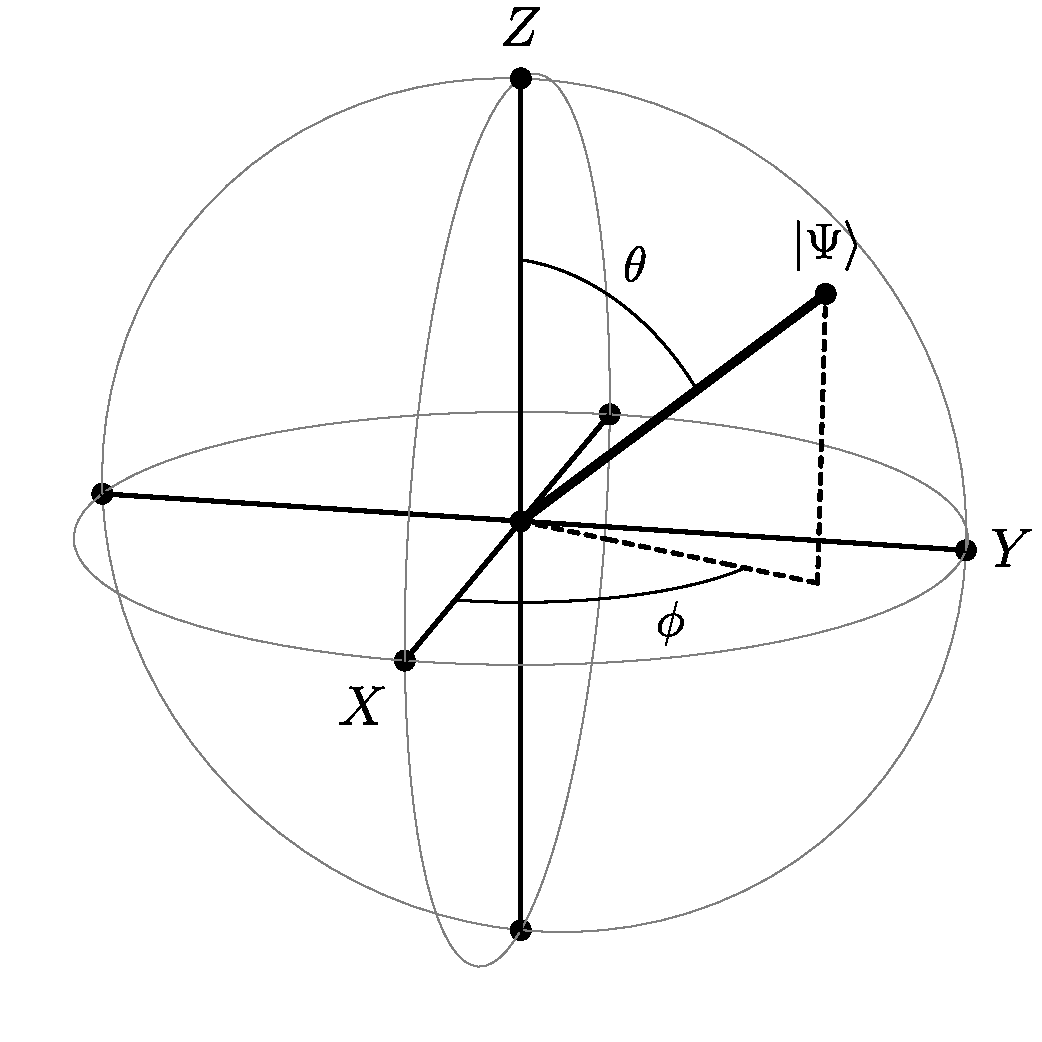
\includegraphics[width=.5\textwidth]{img/blochSphere.pdf}
\caption{The Bloch sphere. The axes correspond to the three Pauli matrices $X$, $Y$ and $Z$, in the sense that rotation around a vector $\vec{n}$ corresponds to the action $U = \exp( -i \vec{n } \cdot \vec{\sigma} / 2)$. Moreover, any point corresponding to a unit vector $\hat{n}$ represents the unique quantum state (up to a global phase) which is the $+1$ eigenstate of $\hat{n}\cdot \vec{\sigma}$. }
\label{fig:blochsphere}
\end{figure}


We often like to visualize the complex, two-dimensional qubit state on a real two-dimensional sphere, called the Bloch Sphere, as depicted in figure \cref{fig:blochsphere}.
%
We represent our qubit states as 
\begin{align}
\ket{\Psi} = \cos(\theta / 2 ) \ket{0} + e^{i \phi} \sin( \theta /2 ) \ket{1}.
\end{align}
We interpret $(\theta, \phi)$ as coordinates on a sphere: $\phi \in (0, 2\pi)$ is the \emph{longitude} (the angle along the equator of the sphere, with respect to some definition of $\phi=0$), and $\theta \in (0, \pi)$ as the \emph{colatitude} (the angle going downwards with respect to the upwards-pointing $Z$-axis). The sphere allows us to graphically represent \emph{actions} on quantum states: a rotation of $\alpha$ radians around a three-dimensional unit vector $\hat{n}$ over the Bloch sphere is equivalent to acting on a qubit state $\ket{\Psi}$ with $U = \exp( -i \alpha \frac{\hat{n} \cdot \vec{\sigma}}{2} )$. A quantum state can also be uniquely defined as an \emph{eigenstate} of these rotations: either as a normalized vector $\hat{n}$ (defining a position on the Bloch sphere), or as the eigenstate with eigenvalue $+1$ of some Hermitian operator $\hat{O} = \hat{n} \cdot \vec{\sigma}$. 

%
%








\section{Modeling interacting qubits}
\label{sec:cmtmodels}
Condensed matter physics deals with the collective behavior of a very large (think $10^{20}$) number of particles. In particular, we will consider spin models, which consist of $N$ particles which are all unable to move, but have certain internal (spin) degrees of freedom. We describe such systems by a vector in the Hilbert space $\mathcal{H} = \bigotimes_{j=1}^{N} \mathcal{H}_j$ with $\mathcal{H}_j = \mathbb{C}^{d_j}$, where $d_j$ is the internal dimension of particle $j$. We use subscripts to indicate on which particle an operator acts.

In the following and in most of this thesis, we restrict to qubits, where $d_j = 2$ for all $j$. For example, the $k$'th Pauli matrix acting on the $j$'th qubit is denoted as
%
\begin{align}
\vec{\sigma}^k_j = \mathds{1}_{2} \otimes \ldots \otimes \mathds{1}_{2} \otimes \vec{\sigma}^k \otimes \mathds{1}_{2} \otimes \ldots \otimes \mathds{1}_{2}.
\end{align}
%
Exceptions are \cref{sec:XXXmodel} and \cref{chap:heisenberg}, where particles of arbitrary spin are allowed. 

\paragraph{} Whenever external forces act on our system's qubits, we call these (local) \textbf{fields}. We describe these by a Hamiltonian term of the form
%
\begin{align}
H = \sum_{j=1}^{N} \vec{B}_j \cdot \vec{\sigma}_j,
\end{align}
%
where $\vec{B}_j \in \mathbb{R}^3$ for all $j$. 

Moreover, the particles may \textbf{interact}, causing their internal states to change as a function of the states of other particles. The set of possible interactions is huge, and most of them may never occur in nature. To keep our focus on the most relevant types of systems, we make two assumptions:
\begin{itemize}
\item The only allowed interactions between particles are $\mathbf{2\textbf{-local}}$. This means that the Hamiltonian is a sum of terms, $H = \sum_j h_j$, where each term $h_j$ is Hermitian and acts non-trivially on at most two particles. 
\item The interactions between the particles are \textbf{symmetric}, which means that the interaction is similar even if the two particles acted on are exchanged.
\end{itemize}
%
The most general form of a \emph{2-local} Hermitian operators on qubits is
\begin{align}
H = \sum_{j < k} \ \ \sum_{p, q \in \{1,2,3\} } \beta^{pq}_{jk} \  \vec{\sigma}^p_j \ \vec{\sigma}^q_k \ \ + \ \ \text{(local fields)}.
\label{eqn:2localham}
\end{align}
The most frequently encountered two-body terms are of the form $X_jX_k$, $Y_jY_k$ and $Z_jZ_k$, and we will shortly discuss the properties of models in which these are the only relevant terms. However, note that many more interactions satisfy the symmetry assumptions, such as $Z_j X_k + X_j Z_k$ or $X_j Y_k - Y_j X_k$. In fact, we will encounter the latter in \cref{chap:pc}. 

The naming conventions of models with a certain choice of $\beta^{pq}$ appear to be somewhat confusing and sometimes contradicting. Therefore, we will always explicitly state the Hamiltonian that we consider. Below, we tease the three models that are addressed later in this chapter: 
\begin{itemize}
\item The Ising-type interaction, of the form $H = \sum_{j<k} w_{jk} Z_j Z_k$ (also sometimes called ZZ interaction), is discussed in \cref{sec:Ising}.
\item The XY model, of the form $H = \sum_{j<k} w_{jk} \left( a  X_j X_k + b Y_j Y_k \right)$. We will focus on the case $a = b$ in \cref{sec:XXmodel}, which is often referred to as the XX or spin hopping model. 
\item \sloppy{The Heisenberg or XYZ type interaction, which is of the form $H= \sum_{j<k} w_{jk} \left( a X_j X_k + b Y_j Y_k + c Z_j Z_k \right)$. If $a,b,c$ are independent, the model is often referred to as XYZ model, but to indicate that some of the three parameters are not independent, one may reflect this by making certain symbols in the model name equal. For example, in \cref{sec:XXXmodel}, we consider the `isotropic' case $a = b= c$, which is often referred to as XXX model. }
\end{itemize}
%


\paragraph{The goal: diagonalizing the Hamiltonian}
Important questions in theoretical physics typically deal with the \emph{ground state} (the vector corresponding to the lowest eigenvalue of $H$), and thermodynamical properties of quantum systems, which can often be derived if one knows the partition function $Z = \text{tr}( e^{-\beta H} )$. On the other hand, for quantum computers we typically assume coherent evolution of pure states, effectively requiring zero temperature. We are then particularly interested in the dynamical properties of the system, which follow from Schr\"{o}dinger's equation. Each of these questions is closely related to finding the eigensystem of the model's Hamiltonian. In this sense, one might generally describe theoretical condensed matter physics, to zeroeth order, as \emph{the science of diagonalizing $k$-local Hermitian matrices}. This is, in general, a difficult task, as the Hilbert space is of dimension $\prod_j d_j$, which grows exponentially with the number of particles\footnote{In physics, the jargon \emph{solving a model} is often used, which vaguely means that the eigensystem of a certain family of Hamiltonians is obtained analytically. Still, with the huge (or possibly infinite) dimensionality of space, an explicit description is often not realistic. Depending on the situation, `solving' could mean as much as finding the ground state and its corresponding energy, finding the free energy, finding the partition function, or expressing the eigenstates in the form of correlation functions or recursive procedures. }.


\subsection{Spin models from graphs}
\label{sec:graphs}
Most well-known theoretical spin models have the same \emph{type} of interactions throughout the system, i.e. $\beta^{pq}_{jk} = w_{jk} \beta^{pq}$, such that the system is completely described by the set $w_{jk}$, indicating the strength of the interaction between two particles, and a global set of $\beta^{pq}$ that determine the interaction type. In such cases, it is intuitive to describe the couplings in the language of graphs, intuitively a drawing of the various spin particles as structureless dots, two of which are connected by a line if and only if they interact. 

Mathematically, we describe a (simple) \textbf{graph} $G = (V,E)$ by its set of vertices $V = \{ j \}_{j=1}^{N}$, corresponding to the set of particles, and the set of edges $E = \{ (j,k) |  \ j,k \in V, \ w_{jk} \neq 0 \}  \subseteq V \times V$, denoting nonzero couplings between spins. More common in this thesis are \textbf{weighted graphs}, $G = (V,E,w)$, which are described by the aforementioned set of vertices $V$ and edges $E$, complemented with a set of \textbf{weights} $w: E \rightarrow \mathbb{R}$. For either type of graph, we may define the \textbf{adjacency matrix} $A_G$: for unweighted graphs, it is a $0/1$-matrix where the entry $(A_G)_{jk}$ is $1$ if and only if $(j,k) \in E$, while for weighted graphs it is the matrix formed by the set of weights $(A_G)_{jk} = w_{jk}$, with $w_{jk} := 0$ if $(j,k) \not \in E$. 
We will sometimes abuse our conventions by assuming that an edge disappears whenever a weight $w_{jk}$ is set to $0$ on purpose, but this should be clear from the context. In general, we allow self-loops, which are edges of the form $(j,j)$. 


Thanks to the mapping to graphs, we can use various notions from graph theory. We denote with $G-j$ the graph $G$ in which the vertex $j$ and all the edges incident to $j$ are removed. The \textbf{degree} of a vertex is the number of edges incident to that vertex, and likewise, the (maximum) degree of a graph is the largest degree found on any of its vertices. A \textbf{bipartite graph} has a vertex set $V$ which can be separated into two disjoint subsets $V_1, V_2$ such that each edge $(j,k) \in E$ must run \emph{between} $V_1$ and $V_2$ (that is, $j \in V_1$ and $k \in V_2$ or vice-versa). 
Two sites $j$ and $k$ are \textbf{connected} if there exists a path of edges between the two sites with nonzero weights, i.e. there exists a sequence $(w_{j,a_1}, w_{a_1,a_2}, \ldots w_{a_n, k})$ of nonzero elements. A graph or subsystem is connected if all pairs of vertices within that graph or subsystem are connected. If a system is not connected, it may consist of non-connected islands. We then use \textbf{connected components} to refer to these islands, i.e. the largest possible subsystems in which all vertices are connected. 

This way, we can define a spin Hamiltonian using a given graph $G=(V,E,w)$ and a type of interaction $\{ \beta^{pq}\}_{p,q = 1}^3$: 
\begin{align}
H &= \sum_{(j,k) \in E} w_{jk} h_{jk},  \label{eqn:hamfromgraph} \\
h_{jk} &= \sum_{p, q \in \{1,2,3\} } \beta^{pq} \ \vec{\sigma}^p_j \ \vec{\sigma}^q_k. \nonumber
\end{align}
Likewise, given a model in which the type of interaction is constant, we can deduce some interaction graph $G$. The weight values $w_{jk}$ arise under various different names in literature, such as \textbf{couplings} or \textbf{interaction strengths}.

In order to represent a Hamiltonian, which has to be Hermitian, the graphs $G$ are required to be \emph{undirected}, meaning that edges always appear in both `directions' ($(j,k) \in E \iff (k,j) \in E$), with opposite weights respecting $w_{jk} = {w_{kj}}^*$. The language of graphs will turn out to be useful at various points throughout this thesis, especially in \cref{part:adiabatic}, where we extend the possible graphs on which certain protocols are known to work.  



\subsection{Diagonalization using symmetries}
Assume our Hamiltonian $H$ admits some symmetry, in the sense that there is a unitary operation $A$ that does not cause the system's energy to change:
\begin{align}
A H A^\dagger = H   \iff [H,A] = 0.
\end{align}
Then, knowing the eigensystem of $A$ (which is often easier to obtain) could help us diagonalize $H$. For each \emph{non-degenerate} eigenvalue of $A$, the corresponding eigenvector must also be an eigenvector of $H$. Eigenvalues of $A$ with higher multiplicities are slightly more involved. Assume we know the eigenbasis of $A$, and we collect all eigenspaces with the same eigenvalue. Then, $A$ is of the form 
\begin{align*}
A = \mu_{1} \mathds{1}_{d_1} \oplus \mu_2 \mathds{1}_{d_2} \oplus \ldots \oplus \mu_J \mathds{1}_{d_J},
\end{align*}
where $\{ \mu_j \}_{j=1}^J$ are the distinct eigenvalues of $A$, each corresponding to an eigenspace of dimension $d_j$. Then $H$, in the same basis, must be of the form
\begin{align}
H = H_1^{(d_1 \times d_1)} \oplus H_2^{(d_2 \times d_2)} \oplus \ldots \oplus H_J^{(d_J \times d_J)},
\label{eqn:blockdiagonal}
\end{align}
where we denote the shape of the matrices $H_j$ in superscripts.
The proof, with a little quantum sauce, is as follows. Let $\ket{\phi}$ be an eigenvector of $A$ such that $A \ket{\phi} = \mu_j \ket{\phi}$. But $\ket{\phi}$ needs not necessarily be an eigenvector of $H$, so perhaps $H \ket{\phi} = \sum_k \alpha_k \ket{k}$ with $\alpha_k = \bra{k} H \ket{\phi}$. What we do know is that $A H \ket{\phi} = \mu_j H \ket{\phi}$, hence whatever states $\ket{k}$ appear in the superposition $\sum_k \alpha_k \ket{k}$, surely they cannot have an $A$-eigenvalue other than $\mu_j$. Thus $\bra{k} H \ket{\phi} = 0$ whenever $\ket{k}$ and $\ket{\phi}$ have a different $A$-eigenvalue, allowing us to derive \cref{eqn:blockdiagonal}. We can summarize the whole argument as \emph{$H$ preserves $A$, so it can never map a quantum number $\mu_j$ to some other quantum number}. 

When $H$ is written in the form of \cref{eqn:blockdiagonal}, we say that $H$ \textbf{block-diagonalizes} into $J$ blocks, with sizes $d_j$, and the subspace corresponding to some eigenvalue $\mu_j$ of $A$ will be called a \textbf{sector} or \textbf{conserved subspace}.

%



\paragraph{}
In fact, any symmetry operator $A$ allows us to give some structure to the eigenstates of $H$, by \textbf{labeling} them as $\ket{ \mu_j , \ldots }$, where we leave some space in the ket for other labels that may be needed to uniquely identify a state. This is a well-known convention in the theory of angular momentum, where $\ket{ s, m }$ labels a state with $\hat{S}_\text{tot}^2$-eigenvalue $s(s+1)$, and simultaneously $\hat{S}_\text{tot}^z$-eigenvalue $m$. Moreover, the computational basis states $\ket{0}$ and $\ket{1}$ can be interpreted as being the $+1$ and $-1$ eigenvectors of the operator $Z$. As theorists, we do not necessarily have a clue what these states actually are, especially if we do not care what $Z$ actually `means' in the real world. In a sense, all we care about is that the states are well-defined with respect to some labeling operator, and that all other operators involved satisfy the correct commutation relations with the labeling operator and with each other. Of course, whenever the Hamiltonian does not have enough symmetries to label all states uniquely, we may resort to the `ugly' approach where a state is defined as the $k$'th eigenvector of $H$ within a conserved subspace. 




%
%
%
%
%
%
%
%
%


%
%




%


\section{The Ising model}
\label{sec:Ising}
Let us now turn to some frequently encountered models. The \textbf{Ising model} on a weighted graph $G = (V,E,w)$ is described by 
\begin{align}
H_\text{Ising} = \sum_{(j,k) \in E} w_{jk} Z_j Z_k %
\label{eq:ising}
\end{align}
which equivalently describes models with interactions of the form $X_j X_k$ or $Y_k Y_k$, up to a local basis transformation. We choose to analyze the model as given in \cref{eq:ising} such that the Hamiltonian is diagonal, and the computational basis states are eigenstates. Note that $H$ is invariant whenever all qubits are flipped, $H_\text{Ising} = X^{\otimes N} H_\text{Ising} X^{\otimes N}$, such that each eigenspace is (at least) two-dimensional.

Whenever $w_{jk} \leq 0$, clearly the ground state is of the form $\alpha \ket{0^{\otimes n}} + \beta \ket{1^{\otimes n}}$, because whenever all qubits are in the same state, the energy of each individual term of $H$ is minimized. The choice of weights is often called \textbf{ferromagnetic} (FM), as the spins tend to align, just as in the material iron. 

Whenever $w_{jk} \geq 0$, the bits prefer to anti-align to minimize each term. This may not always be possible: whenever $G$ has a \emph{cycle} of odd length, not all neighboring spins can anti-align. In such cases, the system is called \textbf{frustrated}, and finding the ground state of such systems is typically a lot harder. 
On the other hand, whenever the interactions form a bipartite graph with parts $V_1$ and $V_2$, then there is a clear ground subspace, spanned by the two N\'{e}el states
\begin{align*}
\ket{\text{N\'{e}el}^\pm} = \ket{0^{\otimes |V_1|}}_{V_1} \ket{1^{\otimes|V_2|}}_{V_2} \pm \ket{1^{\otimes |V_1|}}_{V_1} \ket{0^{\otimes|V_2|}}_{V_2}.
\end{align*}
We call such systems \textbf{anti-ferromagnetic} (AFM) for the tendency of the spins to anti-align. 

Despite its simplicity, even this fairly classical model is notoriously hard to completely solve. The 1D chain is `easy', in the sense that it is efficiently solvable by a Jordan-Wigner mapping to free fermions (see below). On the other hand, finding the ground state or partition function of the 3D grid with local fields is equivalent to solving NP-complete problems \cite{Istrail2000}, so it is unlikely that a closed-form solution exists. Between these two extremes, there are many intermediate cases, many of which are unsolved open problems \cite{McCoy2012}.
%


\section{The XX model and free fermions}
\label{sec:XXmodel}
The \textbf{XX model}, or spin hopping model, on a weighted graph $G = (V,E,w)$, is described by 
\begin{align}
H_\text{XX} &= \frac{1}{2} \sum_{(j,k) \in E} w_{jk} \left( X_j X_k + Y_j Y_k \right)   \label{eqn:Hxx} \\
&= \sum_{(j,k) \in E} w_{jk} \left( \sigma^+_j \sigma^-_k + \sigma^-_j \sigma^+_k \right)  \nonumber
\end{align}
The model's name XX refers to the two different interaction terms, $X_jX_k$ and $Y_jY_k$ having equal amplitude - a model with different scalars in front of the $X$ and $Y$ parts would be called XY model. For some extra confusion, some literature refers to \cref{eqn:Hxx} as XY model \cite{Christandl2004,Ohshima2007}. 


First of all, notice that the total $z$-magnetization $Z_\text{tot} = \sum_j Z_j$ is conserved,
\begin{align*}
[ H_\text{XX}, Z_\text{tot} ] = 0
\end{align*}
hence the Hamiltonian decomposes into blocks of constant number of `spin ups'. We use the term \textbf{Hamming weight} to denote the number of qubits that are in the state $\ket{1}$. All $H_\text{XX}$ really does is making spin up excitations `hop' towards empty (spin down) neighboring sites. The form of $H_\text{XX}$ is reminiscent of free fermion hopping, except that the spin operators $\sigma_j^\pm$ at different sites commute rather than anti-commute. 

As first described by Lieb, Schultz and Mattis \cite{Lieb1961}, if we restrict ourselves to working on an open chain $(G = P_N)$, the model can be solved analytically by using the Jordan-Wigner transformation \cite{Jordan1928}. We define
\begin{align}
f^\dagger_j = [ \prod_{k < j} Z_{k} ] \sigma_j^-, \ \ f_j = [ \prod_{k < j} Z_{k} ] \sigma_j^+,
\end{align}
where $f_j$ now obey precisely the canonical anti-commutation relations that are normally associated to fermionic particles:
\begin{align}
\{ f_j, f^\dagger_k \} = \delta_{jk}, \quad 
\{ f_j, f_k \} = 0, \quad  \{ f^\dagger_j, f^\dagger_k \} = 0.
\end{align}
The product $\prod_{k < j} Z_{k}$ makes the operators highly non-local, forming the so-called \emph{string operator} that trails the raising and lowering operators over the graph. Intuitively, the string counts the number of fermions one has to `jump over' in order to create or annihilate a fermion at position $j$, which in turn leads to proper anti-commutative properties. On a general graph, this would lead to a rather involved Hamiltonian, but it happens that on the open chain, the string operators of $\sigma^+_j$ and $\sigma^-_{j+1}$ precisely cancel. \cref{eqn:Hxx} then becomes
\begin{align}
H_\text{ff chain} = \sum_{j=1}^{N} w_{j, j+1} \left( f^\dagger_j f_{j+1} + \text{h.c.} \right).
\label{eqn:ffchain}
\end{align}
The latter is an example of a \textbf{free fermion} model, in which individual particles jump around over the lattice, without explicitly affecting one another. Clearly, the particles are \emph{non-interacting}, and we may just as well treat the system as if just a single particle is present in it. This reduces the dimensionality of our problem from $2^N$ down to just $N$, making it efficient to solve. In fact, our treatment below works for general models of free fermions hopping on any weighted graph $G$ (with, of course, $w_{jk} = w_{kj}^*$):
\begin{align}
H_\text{ff} = \sum_{j,k=1}^N w_{jk}  f^\dagger_j f_{k}
\label{eqn:freefermion}
\end{align}

Mathematically, our goal is to massage \cref{eqn:ffchain} into the form 
\begin{align}
H_\text{ff diag} = \sum_{k=1}^N \lambda_k c^\dagger_k c_k\
\label{eqn:ff_diag}
\end{align}
through a canonical basis transformation
\begin{align}
c^\dagger_k= \sum_{j=1}^N U_{j,k} f^\dagger_j, \quad c_k = \sum_{j=1}^N (U^\dagger)_{k,j} f_j, \\
f^\dagger_j= \sum_{k=1}^N (U^\dagger)_{k,j} c^\dagger_k, \quad f_j = \sum_{k=1}^N U_{j,k} c_k.
\end{align} 
where $U$ is a unitary matrix we get to pick ourselves, and the operators $c^\dagger$ are often said to create (fermionic) \textbf{modes} or \textbf{quasi-particles}. The effect of plugging this transformation into \cref{eqn:freefermion} is
\begin{align*}
H_\text{ff} &= \sum_{j,k = 1}^N \ \sum_{k_1, k_2 = 1}^N w_{jk} U^\dagger_{k_1,j} U_{k,k_2} c^\dagger_{k_1} c_{k_2} \\
 &= \sum_{k_1, k_2 = 1}^N \left( U^\dagger w U \right)_{k_1, k_2} c^\dagger_{k_1} c_{k_2}.
\end{align*} 
To retrieve the form of \cref{eqn:ff_diag}, we require $( U^\dagger w U )_{jk} = \delta_{jk} \lambda_k$. In other words, the basis transformation amplitudes $U_{jk}$ are precisely the entries of the matrix $U$ that \emph{diagonalizes} $w$. In fact, we could have seen this in a more handwaving way too: the Hamiltonian $H_\text{ff}$ block-diagonalizes into sectors with fixed particle number. Restricting to just a single fermion, the Hamiltonian is precisely the matrix $w$. Clearly, the single-particle energies are the eigenvalues of $w$, and the eigenstates correspond to the eigenvectors of $w$.

Having obtained \cref{eqn:ff_diag}, we may now read off the full eigensystem of $H_\text{XX}$. The eigenstates are of the form 
\begin{align}
\ket{\vec{s}}_c &= ( c^\dagger_{1} )^{s_1}  ( c^\dagger_{2} )^{s_2}  \ldots (c^\dagger_N )^{s_N} \ket{0} 
\label{eqn:eigenmodes}
\end{align}
where $s \in \{0,1\}^N$ is a binary string of length $N$ that denotes \emph{which fermionic modes are absent/present}, and $\ket{0}$ is the fermionic vacuum. The subscript of a ket, such as the $c$ in $\ket{\vec{s}}_c$, denotes the \emph{basis} in which the state is given -- we will use this convention throughout this thesis. The energies of the eigenstates are \emph{sums of single-particle energies}:
\begin{align}
H_\text{ff} \ket{\vec{s}}_c  = \left( \sum_{k=1}^N  s_k \lambda_k \right) \ket{\vec{s}}_c.
\end{align}
One might wonder what a state like $\ket{\vec{s}}_c$ looks like in our `natural'  basis, consisting of local fermionic operators $f$ or even going back to spins $\sigma^\pm$. The product of $c^\dagger$ operators in \cref{eqn:eigenmodes} leads to a huge number of terms, each with the same number of $f$ operators applied to $\ket{0}$. Many of these terms will drop out, because any two fermions at the same location are not allowed ($f_j^\dagger f_j^\dagger = 0$). In fact, the result is a weighted sum over \emph{all combinations of unique $f$ operators}, weighted by some function $F$:
\begin{align*}
\ket{ \vec{s} }_c  = \sum_{ z \in \{0,1\}^N } F( \vec{s}, \vec{z} )    \ket{  \vec{z}  }_f.
\end{align*}
The function $F(\vec{s}, \vec{z})$ is a large sum, in which each term is a product of weights $U_{j,k}$. These are precisely the matrix elements obtained when converting a certain $c_k$ operators (given by $\vec{s}$) into one of the possible  $f_j$ operators (described by $\vec{z}$), except for the minus signs that appear when re-ordering the $f$ operators. This happens to correspond precisely to taking the determinant! Hence, we claim that
\begin{align*}
F( \vec{s} , \vec{z} ) = | U_{\vec{s}, \vec{z}} |,
\end{align*}
where $| \cdot |$ denotes the determinant of a matrix. With $U_{\vec{s}, \vec{z}}$ we denote the matrix $U$ with only the rows $k$ kept corresponding to $s_k = 1$, and likewise, where columns $j$ are kept only if $z_j = 1$. We define the determinant of a non-square matrix to be zero, such that any strings $\vec{z}$ that do not have the same Hamming weight (i.e., number of particles) as $\vec{s}$ drop out. The function $F$ is closely related to the \textbf{Slater determinant}, which is used to represent that second quantized Fock states in first quantized notation \cite{Altland2010}.

In \cref{chap:krawtchouk}, we will put the techniques discussed here to creative use: we try to make JW string operators that cover precisely half of the system, such that highly non-local terms appear in the Hamiltonian. The time-evolution of such Hamiltonians would allow one to make fast multiqubit logic gates that would otherwise take a large circuit. To quantify precisely how long the gate takes, we need to calculate the matrix element of the JW string sandwiched between different eigenstates. By representing these eigenstates as Slater determinants, we obtain analytical expressions for the matrix elements, again in the form of determinants of sub-matrices of $U$. 


\section{The XXX model, or Heisenberg model}
\label{sec:XXXmodel}
For this model, we consider not only qubits (which are spin-$\frac{1}{2}$ particles), but also more general particles of arbitrary spin. Recall that for a \emph{single} spin particle, the three spin operators, $\vec{S} = \{ \hat{S}^x, \hat{S}^y, \hat{S}^z \}$, are Hermitian operators acting on the spin vector space $(s) = \mathbb{C}^d$, of dimension $d =2s+1$. The spin operators have unique eigenvalues $\{-s, -s+1, \ldots s-1, s\}$, and as usual, we choose to work in the basis in which $\hat{S}^z$ is diagonal. The basis vectors are thus uniquely identified by the eigenvalue $m$ of $\hat{S}^z$. Moreover, the operator $\hat{S}^2 = (\vec{S})^2 = \vec{S} \cdot \vec{S}$ commutes with each of the three spin operators and has a single eigenvalue, $s(s+1)$. In fact, one may use this operator to define the value $s$ of a spin representation $(s)$. Note the subtle difference between the many appearances of the letter $S$. For clarity, we adhere to the convention that spin-related scalars (often eigenvalues) get lowercase symbols. Spin operators are capitalized and wear a hat, and spin vectors are overlined with an arrow. 

The (isotropic) Heisenberg model, or XXX model, can be defined on a set of $n$ spin particles, each with a possibly different spin. The term isotropic refers to the weights $\beta^{pq}$ being equal in each of the three spin directions $x$, $y$ and $z$, which is not to be confused with \emph{homogeneous}, typically used to indicate that there is no spatial variation in the couplings $w_{jk}$. We let subscripts denote the particle (or set of particles) on which an operator acts. For example, particle $j$ has a total spin $s_j$. Given a weighted graph $G = (V,E,w)$, the Heisenberg model is described by 
\begin{align}
H_\text{H} &=  \sum_{(j,k) \in E} w_{jk} \vec{S}_j \cdot \vec{S}_k 		\nonumber \\
&=  \sum_{(j,k) \in E} w_{jk} \left( \hat{S}^x_j \hat{S}^x_k + \hat{S}^y_j \hat{S}^y_k + \hat{S}^z_j \hat{S}^z_k \right)  	\label{eqn:intro_heisenberg} \\
&= \sum_{(j,k) \in E} w_{jk} \left( \frac{1}{2} \left[ \hat{S}^+_j \hat{S}^-_k + \hat{S}^-_j \hat{S}^+_k  \right] + \hat{S}^z_j \hat{S}^z_k \right).  \nonumber
\end{align}
%
Here, the spin raising and lowering operators are defined as $\hat{S}^\pm = \hat{S}^x \mp i \hat{S}^y$. Also note that, specifically for spin-$\frac{1}{2}$ particles, the interaction can be written as a SWAP-operation, up to addition by $\mathds{1}$:
\begin{align}
\frac{1}{2} \left( X_j X_k + Y_j Y_k  +  Z_j Z_k + \mathds{1}_4 \right) = \begin{pmatrix}
1 & 0 & 0 & 0 \\
0 & 0 & 1 & 0 \\
0 & 1 & 0 & 0 \\
0 & 0 & 0 & 1 \\
\end{pmatrix}.
\label{eqn:heisenbergswap}
\end{align}

Owing to the inner product between the vectors of spin operators $\vec{S}$ in the top line of \cref{eqn:intro_heisenberg}, $H_\text{H}$ depends only on the \emph{relative} orientation of the spin particles, but does not reference any absolute direction. Hence, we expect the system to be invariant under arbitrary global rotations around the $x$, $y$ and $z$-axis, where all spin particles rotate in the same way. We make this precise as follows. We define total spin operators
\begin{align}
\hat{S}_\text{tot}^x = \sum_{j=1}^n \hat{S}^x_j, \quad \hat{S}_\text{tot}^y = \sum_{j=1}^n \hat{S}^y_j, \quad \hat{S}_\text{tot}^z =  \sum_{j=1}^n \hat{S}^z_j,
\end{align}
which we sometimes like to take together as $\vec{S}_\text{tot} = ( \hat{S}_\text{tot}^x, \hat{S}_\text{tot}^y, \hat{S}_\text{tot}^z )$ (note the difference with $\vec{S}_j$ of a \emph{single} spin!). These are generators of global rotations of the form $U(\vec{\theta})^{\otimes n}$, with $U(\vec{\theta}) = \exp(-i \vec{S} \cdot \vec{\theta} )$.  %
The Hamiltonian is actually invariant under these rotations, because 
\begin{align}
[H_\text{H} , \hat{S}_\text{tot}^\alpha ] = 0, \quad \alpha \in \{ x, y, z\}.
\end{align}
In proving the above, we save ourselves some work by noting that  $H_\text{H}$ is symmetric under any permutation of the labels $x, y, z$, hence we choose to only show commutativity for the $z$-component. This, in turn, can be seen from the bottom line of \cref{eqn:intro_heisenberg}. The terms $\hat{S}^+_j \hat{S}^-_k + h.c.$ are reminiscent of hopping in the XX model (\cref{sec:XXmodel}) and conserve the total $z$-magnetization. Also the terms $\hat{S}^z_j \hat{S}^z_k$ clearly commute with $\hat{S}_\text{tot}^z$. Altogether, we find that indeed the number of spin excitations in \emph{any} direction is conserved, and equivalently, that the Hamiltonian is symmetric under rotations generated by any $\hat{S}^\alpha_{\text{tot}}$. 

Using the previous result, we also find that 
\begin{align}
[H_\text{H} ,  ( \hat{S}_\text{tot} )^2  ] = 0,
\end{align}
where $\hat{S}_\text{tot}^2 = \vec{S}_\text{tot} \cdot \vec{S}_\text{tot}$. Having found two operators that commute with the Hamiltonian, we know that we can label our eigenstates as $\ket{s, m}$, where $s$ is some eigenvalue related to $\hat{S}_\text{tot}^2$ (which we will come back to in a bit), and $m$ is the $z$-magnetization eigenvalue of $\hat{S}_\text{tot}^z$. Note that we can not do better at this point, because $\hat{S}_\text{tot}^x$ and $\hat{S}_\text{tot}^y$ do not commute with $\hat{S}_\text{tot}^z$.

\paragraph{}
Now, what precisely are these subspaces, labeled by $s$ and $m$, which are invariant under the actions of $\hat{S}_\text{tot}^z$ and $\hat{S}_\text{tot}^2$? We saw that the rotations $U(\vec{\theta})$ generated by $\vec{S}_\text{tot}$ commute with $H$. Intuitively, these operators rotate the system as a whole, leaving relative angles unchanged, hence preserving the system's energy. The system behaves \emph{almost} as if it collectively forms a single spin particle, with a potentially huge total spin. This total spin is precisely the variable $s$ of the collective system. 

In the following, we resort to the representation theory of spin particles to make this statement more precise. We will find that the total space spanned by $n$ `real' spin particles decomposes into various `virtual' spin particles. The decomposition is such that the operators $\hat{S}^\alpha_\text{tot}$ rotate these virtual spins as if these are elementary spin particles, and in particular, do not mix the states of different virtual particles. The particles each have a well-defined spin $s$, which can be retrieved by acting on the spin states with the operator $\hat{S}^2_\text{tot}$. 

Exploiting that $(s)$ is an irreducible representation of the algebra $\textbf{su}(d)$, we can combine multiple spin particles, taking the tensor products of spin spaces $(s_1), (s_2)$ to form the new space $(s_1) \otimes (s_2)$. Within the new space, new irreducible representations of $\textbf{su}(d')$ can be found, which look precisely as the single-particle spaces $(s)$ that we are used to. The precise formulation is given by the \textbf{Clebsch-Gordan rule}:
\begin{align}
(s_1) \otimes (s_2) = \bigoplus_{s = |s_1 - s_2|}^{s_1 + s_2} (s).
\label{eqn:intr_clebschgordanrule}
\end{align}
This rule can be applied iteratively to obtain the decomposition of the space of $n$ spin particles, each having spin $s_1, s_2, \ldots, s_j, \ldots, s_n$:
\begin{align}
\bigotimes_{j=1}^n (s_j) = \bigoplus_{s} N_{s_1, s_2, \ldots s_n}^{s} \ (s).
\label{eqn:intr_clebschgordan}
\end{align}
Here, $N^s_{s_1, s_2, \ldots s_n}$ denotes the multiplicity with which the spin representation $(s)$ appears. In other words, upon combining \emph{real} spin particles, we retrieve a huge number of \emph{virtual} spin particles. This structure of the total Hilbert space is depicted in \cref{fig:clebschgordan}. In each of these spaces $(s)$, the spin operators $\vec{S}_\text{tot}$ act just like how $\vec{S}$ would act on a normal, isolated particle of total spin $s$. The operator $\hat{S}_\text{tot}^2$ now plays a more interesting role: it probes spin of the virtual particle, returning the eigenvalue $s(s+1)$. 

\begin{figure} 
\begin{tabular}{m{0.44\textwidth} m{0.44\textwidth}}
  \vspace{0pt} 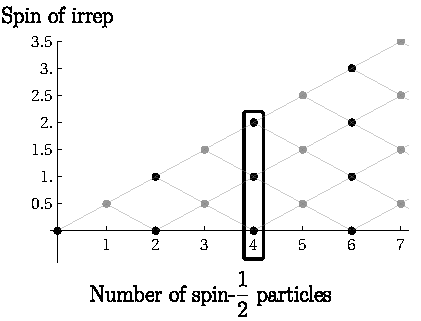
\includegraphics[width=.46\textwidth]{img/ClebschGordanDiagram.pdf} &
  \vspace{0pt} 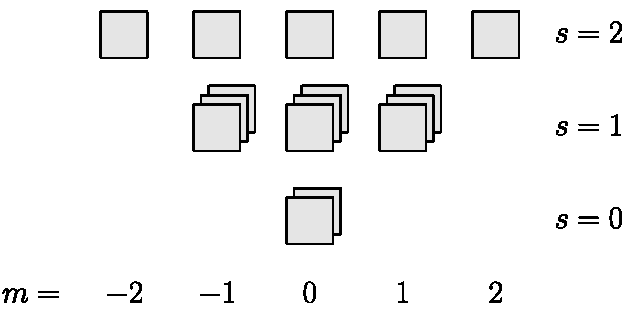
\includegraphics[width=.43\textwidth]{img/HeisenbergSubspaces_flat.pdf} 
\end{tabular}
\caption{The irreducible (spin) subspaces for a system of $n$ spin-$\frac{1}{2}$ particles. Left: The space $(s)^{\otimes n}$ ($n$ labeled horizontally) decomposes into spaces of spin $s'$ (vertically) by iterative application of \cref{eqn:intr_clebschgordanrule}. The multiplicities $N^{s'}_{\frac{1}{2}, \ldots \frac{1}{2}}$ are given by the number of paths leading to a point $(n,s)$ starting at $(0,0)$. Right: For $n=4$, eigenstates of $H_\text{H}$ have a fixed total spin $s =0, 1$ or $2$ (vertical), whose $2s+1$ basis states can be labeled by their $z$-magnetization $m$ (horizontal). In this case, the multiplicities of the spin spaces are 2, 3 and 1, respectively, which we depict as copies closely behind one another. This way, each square corresponds to a single state.   }
\label{fig:clebschgordan}
\end{figure}



Let us now turn back to the Heisenberg Hamiltonian of \cref{eqn:intro_heisenberg}, with the aim of diagonalizing it. We know that it commutes with $\hat{S}_\text{tot}^2$, which takes the form 
\begin{align*}
\hat{S}_\text{tot}^2 =  \bigoplus_{s} s(s+1) \ \mathds{1}_{(2s+1) \times  N^s_{s_1, \ldots, s_n}}  ~ .
\end{align*}
Moreover, $H_\text{H}$ commutes with $\hat{S}_\text{tot}^z$, which depends only on the Hamming weight of a state. This way, we can see that $H_\text{H}$ decomposes into blocks, each acting on a subspace of fixed eigenvalues $s,m$. Note that the energy of two states with the same values of $s,m$ \emph{can} actually differ, because there may be multiple irreps with the same $s$. On the other hand, within each irrep $(s)$, due to rotational invariance, the energies are equal for each $m$. 

\paragraph{Ferromagnetic case} Just as with the Ising model, we can easily guess \emph{some} of the ground states when couplings are \emph{ferromagnetic}, $w_{jk} \leq 0$. We already noted that neighboring states that have their spin aligned are energetically favorable. Indeed, we find that each two-body interaction in \cref{eqn:intro_heisenberg} is minimized whenever all spins $j$ have either maximum $z$ magnetization $\ket{m=s_j}$ or minimum $z$ magnetization $\ket{m=-s_j}$. These states have the minimum and maximum possible total $z$-magnetization, $m = \pm \sum_j s_j$, and hence must correspond to the unique spin representation with the highest possible spin, $(s= \sum_j s_j)$. By rotational symmetry, all other values of $m$ share the same energy under $H_\text{H}$, hence the ground space is spanned by \emph{at least} the states $\ket{ s= \sum_j s_j, m }$. We have not shown that these are the \emph{only} ground states - there could in principle be states with different $s$ with the same ground energy. %


\paragraph{Anti-ferromagnetic case} Equivalently, we may consider the \emph{anti-ferromagnetic} setting of couplings, where $w_{jk} \geq 0$. On a frustration-free graph, one might naively think that the N\'{e}el state is again a lowest energy state, but one can check that the bottom line in \cref{eqn:intro_heisenberg} does not allow this state as an eigenstate (due to the hopping terms $ \hat{S}^+_j \hat{S}^-_k $). Lieb and Mattis \cite{Lieb1962} found a more concrete description of the ground state as long as the system's graph is a \emph{bipartite} graph. On these graphs, we define the spin imbalance $g$ as the difference between the maximum allowed spin of each part: 
\begin{align}
g = \sum_{j \in V_1} s_j - \sum_{j \in V_2} s_j = \max s_{V_1} - \max s_{V_2}.
\label{eq:imbalance}
\end{align}
Note that spin imbalances can be simply added when combining spin systems: if subsystems have spin imbalances $g_1, g_2, \ldots$, then the combined system has a spin imbalance $g = \sum g_j$. The result by Lieb and Mattis can then be stated as follows:
%
\begin{theorem*}[Lieb-Mattis]
Let $G$ be a weighted, connected, bipartite graph, whose weights are anti-ferromagnetic ($w_{jk} \geq 0$). Then, the ground state of $H_\text{H}$ has total spin $s  = g$. Moreover, if $E(s)$ denotes the \emph{lowest} energy of the subspace with fixed total spin $s$, then 
\begin{align*}
E(s+1) > E(s)  &\text{ for all } s \geq g, \\
E(g) < E(s)  &\text{ for all } s < g.
\end{align*}
\label{thm:LiebMattis}
\end{theorem*}
%
%
A cartoon of this result is shown in \cref{fig:energyPerStot}. The result shows that, in particular, if the maximum allowed spins on $V_1$ and $V_2$ are equal, then the ground state has $s = 0$, i.e. it is a singlet and non-degenerate. If  $s_{V_1} = s_{V_2} +\frac{1}{2}$, then the ground state has $s = \frac{1}{2}$ and the ground state is 2-dimensional (allowing one to encode a qubit), and so forth.

\begin{figure}
\centering
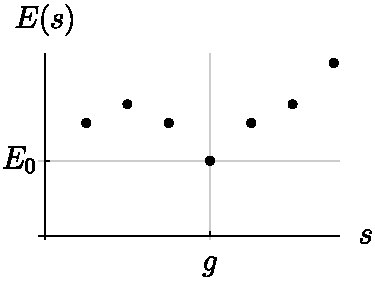
\includegraphics[width=.4\textwidth]{img/energyPerSBlack.pdf}
\caption{A plot of a mock function $E(s)$ that would be in line with the Lieb-Mattis theorem. As long as $s > g$, then the function is strictly increasing. If $s < g$, then we cannot say anything about the ordering of energies, but at least we know all energies are higher than the ground state occurring at $s = g$. }
\label{fig:energyPerStot}
\end{figure}

\begin{proof}
The proof of the theorem uses the following argument. I recommend keeping the RHS of \cref{fig:clebschgordan} in mind for a better understanding.
\begin{enumerate}

\item \textbf{Within the subspace of fixed $(\Stot)^z = m$, there is a unique ground state $\ket{\psi^m_\text{gs}}$ with all-positive coefficients (in a specific basis).} 

Consider the rotation $U = \prod_{j \in V_1} \hat{S}^z_j$. Then, $U H_\text{H} U^\dagger$ looks as follows in the computational basis: all diagonal elements (from terms $\hat{S}^z_j \hat{S}^z_k$) are \emph{positive} and all off-diagonal elements (from $\hat{S}^-_j \hat{S}^+_k + \text{h.c.}$) are \emph{negative}. Hence, within each block of fixed $m$, the \emph{unique} lowest energy state is a superposition of basis states with only \emph{positive} coefficients (by the Perron–Frobenius theorem). We denote this state by $\ket{\psi^m_\text{gs}}$. The state has nonzero overlap with \emph{all} computational basis states with $(\Stot)^z = m$, because the hopping terms map to all states with the same $m$, unless some sites are disconnected. Because it is impossible to make two orthogonal states with positive amplitude on every single basis element, this ground state must be unique (per value of $m$). 


\item \textbf{If $\ket{\psi^m_\text{gs}}$ has $s = m$, then $E(s + 1) > E(s)$}. 

Note that the subspace with total spin $s$ includes all $m$ up to and including $s$. This means that the lowest-energy state with fixed $m$, $\ket{\psi^m_\text{gs}}$, could possibly lie in all subspaces with total spin $s \geq m$. If $\ket{\psi^m_\text{gs}}$ lies in the space $\stot = m$, then $\stot+1$ must contain only states with a strictly higher energy. 

Graphically, on the LHS of \cref{fig:clebschgordan}, if $\ket{\psi^m_\text{gs}}$ has $\stot = m$, then the ground state of an $m$-column occurs in the lowermost row. All higher rows also contain states with the same $m$, but they happened to not hold the ground state, hence these rows must have strictly higher energies. Thus, $E(s+1)$ must be larger than $E(s)$. 


\item \textbf{For a special Hamiltonian $\tilde{H}$, for all $\stot \geq g$, the state $\ket{\psi^m_\text{gs}}$ has $\stot = m$}. 
Let $\tilde{H}$ be the Hamiltonian of the isotropic Heisenberg where all allowed edges have weight $w_{jk} = 1$ (recall that the graph was assumed to be bipartite): 
\begin{align*}
\tilde{H} = \sum_{j \in V_1,\  k \in V_2} \vec{S}_j \cdot \vec{S}_k = \vec{S}_{V_1} \cdot \vec{S}_{V_2}.
\end{align*}
Here, we defined $\vec{S}_{V_x} = \sum_{j \in V_x} \vec{S}_j$.  
Note that $\vec{S}_\text{tot} = \vec{S}_{V_1} + \vec{S}_{V_2}$ and hence $\vec{S}_\text{tot} \cdot \vec{S}_\text{tot} = (\vec{S}_{V_1})^2 + (\vec{S}_{V_2})^2 + 2 \vec{S}_{V_1} \cdot \vec{S}_{V_2}$. Therefore, we can write $\tilde{H}$ in a form in which all operators mutually commute: 
\begin{align}
\tilde{H} = \frac{1}{2} \left( \Stot^2 - (\vec{S}_{V_1})^2 - (\vec{S}_{V_2})^2 \right)
\label{eqn:htilde}
\end{align}
Then, using $s_{V_1}$ and $s_{V_2}$ to denote the spin eigenvalues related to $(\vec{S}_{V_1})^2$ and $(\vec{S}_{V_2})^2$, the energies $\tilde{\varepsilon}$ of $\tilde{H}$ depend only on the spin values as follows:
%
\begin{align*}
\tilde{\varepsilon} = \frac{1}{2} \left( s(s+1) - s_{V_1} (s_{V_1} + 1) - s_{V_2} (s_{V_2} + 1) \right).
\end{align*}
%
To find the ground state, one has to compromise between minimizing $\stot$ and maximizing $s_{V_{1,2}}$. Due to the form of the Clebsch Gordan rule, \cref{eqn:intr_clebschgordanrule}, we can distinguish two cases. Firstly, if $s \geq g$, then for any choice of $s_{V_{1,2}}$, the minimum possible total spin is $s = |s_{V_1} - s_{V_2}|$. We will now argue that the lowest energy always occurs when $s_{V_{1,2}}$ are maximal.
%
Without loss of generality, assume $s_{V_{1}} > s_{V_{2}}$. Then, the energy simplifies to $\tilde{\varepsilon} = -s_{V_{1}} s_{V_{2}} - s_{V_{2}}$. Clearly, the spins on each part should be maximized, and $s=g= | \max s_{V_1} - \max s_{V_2} |$. The state $\ket{\psi^m_\text{gs}}$ lives in the sector with the lowest possible energy for the given $m$, which is, in this case, $s=m$. 

A second case occurs when $s < g$. In this case, the rule $s > |s_1 - s_2|$ tells us that $s_{V_{1,2}}$ cannot be optimized, and it is unclear in what spin sector the state $\ket{\psi^m_\text{gs}}$ would live. All we know is that surely $s<g$ is suboptimal - the ground state will not be in this sector. 

\item \textbf{The state $\ket{\psi^m_\text{gs}}$ of a general $H_\text{H}$ has the same total spin $\stot$ as $\ket{\psi^m_\text{gs}}$ of $\tilde{H}$.}

We found that for any choice of weights $w$ that satisfy the assumptions, the state $\ket{\psi^m_\text{gs}}$ has only positive entries (in some basis). This holds for $\ket{\psi^m_\text{gs}}$ of $H_\text{H}$ as well as for $\tilde{H}$, meaning that both states have nonzero overlap. Therefore, the value of $\stot$ of \emph{any} $\ket{\psi^m_\text{gs}}$ must be the same as whichever holds for $\tilde{H}$. 
\end{enumerate}
%
Putting it all together, we have to distinguish the two cases again. If we are interested in the sector $s \geq g$, then \textbf{3.} and \textbf{4.} state that $\ket{\psi^m_\text{gs}}$ has $s=m$, and by \textbf{2.} the energy as a function of total spin $E(s)$ must be strictly increasing. On the other hand, when $s<g$, we are unable to say anything about $E(s)$. All we know is that the global ground state is not in these sectors. 
\end{proof}

\paragraph{}  In \cref{chap:heisenberg}, we will elaborate on these (fairly old) results in the more modern context of adiabatic state transfer, where the uniqueness of each $\ket{\psi^m_\text{gs}}$ guarantees an adiabatic protocol to work without encountering degeneracies. 









\chapter{Manipulating quantum states}

%

%


%
%
%
%





\section{How to form a quantum gate}
\label{sec:manipulate}
%

We start by sketching the most elementary methods to change a quantum state. The changes occurring to a quantum state $\ket{\psi} \in \mathcal{H}$ in a closed system (i.e. there is no interaction with the environment) are captured by the Hamiltonian $H$. This operator plays a dual role in quantum mechanics. Firstly, $H$ is the Hermitian observable whose eigenvalues determine the \textbf{energy} 
%
$\lambda_j$ of an eigenstate $\ket{\psi_j}$,
\begin{align*}
H \ket{\psi_j} = \lambda_j \ket{\psi_j}.
\end{align*}
Secondly, the Hamiltonian uniquely defines a trajectory of a state through the Hilbert space as a function of time, through \textbf{Schr\"{o}dinger's equation}\footnote{We assume units such that $\hbar = 1$.} (SE)
\begin{align}
\partial_t \ket{\Psi(t)} = -i H(t) \ket{\Psi(t)}.
\end{align}
Note the different notation between $\ket{\psi_j}$ for eigenstates and $\ket{\Psi(t)}$ for time-evolving states, which are generally \emph{not} eigenstates. SE guarantees that $\ket{\Psi(t)}$ evolves in a \emph{unitary} way, making sure that the state is normalized at all times, and that initially orthogonal states remain orthogonal at any time $t$. We can thus describe the time-evolution of a state as 
\begin{align*}
\ket{\psi(t)} = U_{t} \ket{\psi(0)}
\end{align*}
where $U_{t}$ is called the (unitary) \textbf{time evolution operator}. Note that we always assume a time evolution to start at $t=0$. A major part of this thesis is devoted to \emph{solving the time-evolution}, i.e. finding $U_t$ with $H(t)$ given, or the inverse \emph{control problem}, where we try to construct a Hamiltonian $H(t)$ which leads to a required time evolution $U_t$, within realistic constraints. 

\paragraph{Solving time evolutions} Sometimes the time-evolution of $H$ is easy to find. For one, if $H$ is time-independent, then 
\begin{align*}
U_t = \exp( -i H t )  \tag{$H$ time-independent}
\end{align*}
where the exponential of a matrix is defined through the Taylor series. This equation is particularly interesting whenever we know the \emph{eigenbasis} of $H$, such that eigenstates merely pick up a \emph{dynamical phase}
\begin{align*}
\ket{\psi_j(t)} = \exp(-i H t ) \ket{\psi_j(0)} = \exp( -i \lambda_j t ) \ket{\psi_j(0)}.
\end{align*}
Of course, finding the eigenbasis itself may be a nontrivial problem. The time evolution is more tricky to solve whenever $H$ is time-dependent, but in \cref{sec:adiabatic,sec:resonantdriving} we present two cases in which such time evolutions can be solved approximately. 

\paragraph{Control problems} Given a unitary $U_t$, one can always find a Hamiltonian $H$ that causes precisely such a unitary time evolution. The solution is $H = \frac{1}{-it} \log( U )$, such that $\exp(-i H t) = U$. 
With this in mind, one might wonder what is so hard about control problems? The problem is that, in general, the solved Hamiltonian $H$ will be highly non-local, and it may be impossible to engineer such Hamiltonians in nature. To enforce properties such as $2$-locality (see \cref{sec:cmtmodels}), one has to resort to time-dependent Hamiltonians, or sequences of unitary steps. 

Practical control problems typically assume a restricted Hamiltonian of the form \cite{Dong2010}
\begin{align}
H(t) = H_\text{bg} + \sum_j f_j(t) H_j,
\end{align}
where $H_\text{bg}$ consists of forces that are always on (and cannot be turned off), whereas various terms $H_j$ can be modulated in amplitude through scalar \textbf{controls} $f_j(t)$. The controls themselves may also be subject to certain restrictions. It should be clear that, with these assumptions, it is much more challenging to find a set of time-dependent control functions $\{ f_j(t) \}$ that precisely lead to the desired unitary evolution $U_t$.


\paragraph{}
Especially in the context of quantum information technology, these control problems have applications in the construction of tiny computational steps on qubits, which are then called \textbf{quantum gates}. To develop some intuition for quantum control, let us consider the toy problem constructing a very simple gate: flipping the state of a single quantum bit, as described by the Pauli operator $X$. The problem is formalized as:
\begin{align}
& \text{Find controls }& \vec{f}(t) &= \{ f_x(t), f_y(t), f_z(t) \} \nonumber \\
& \text{such that the system } &  H(t) &= H_\text{bg} + f_x(t) X + f_y(t) Y + f_z(t) Z    \label{eq:controlproblem} \\
& \text{causes the evolution } & U_{t} &= X. \nonumber
\end{align}

\subsection{Quenches}
\label{sec:quench}

A \textbf{quench} is a sudden (often instantaneous) change to a Hamiltonian. In particular, a system that was initially in an eigenstate, may not be after the quench, leading to a non-trivial time evolution. Quenches typically assume that the Hamiltonian, as a function of time, is piecewise time-independent (i.e. constant), but this is no hard rule. We will often use the word `quench' to mean that a Hamiltonian is turned `on' at $t=0$, and is then turned `off' at some later time $T$, leading to a well-defined time evolution $U_T = \exp( -i H T)$. 
%

To form a bit-flip, we observe that the Hamiltonian $H = \Omega X$ is precisely the field which \emph{generates} the unitary $U = X$ after a time $t = \frac{\pi}{2 \Omega}$,
\begin{align*}
U_{t} = \exp(-i \Omega X t ) = \cos( \Omega t ) \mathds{1} + \sin( \Omega t ) X,
\end{align*}
where the factor of $2$ comes from the eigenvalue gap of $X$. The evolution of an initial state $\ket{\Psi(0)} = \ket{0}$ is depicted on the Bloch sphere in \cref{fig:xgate_blochsphere}. 

In general, any time-independent quench on a two-level system can be described as a rotation of the form
\begin{align}
U_{\hat{n}}(t) = e^{-i t \vec{n} \cdot \vec{\sigma} } = \cos( n t ) \mathds{1} - i \sin( n t ) \left( \frac{ \vec{n} }{n} \right) \cdot \vec{\sigma}  \label{eqn:tlsrot} \\
\text{with } \vec{n} = \begin{pmatrix} n_x \\ n_y \\ n_z \end{pmatrix}, 
\quad n = | \vec{n} | = \sqrt{ n_x^2 + n_y^2 + n_z^2 }. \nonumber
\end{align}
Such a rotation around the Bloch sphere by an angle $\theta = \frac{n t}{2}$ is sometimes referred to as a $\theta
$-pulse. For example, the $X$-gate we discussed before is a $\pi$-pulse around the vector $\vec{n} = (1,0,0)^T$. 

We conclude that the problem in \cref{eq:controlproblem} with $H_\text{bg} = 0$ can be straightforwardly solved by choosing $\vec{f}(t) = \{ \Omega, 0, 0 \}$, with $\Omega = \frac{1}{2}$. 
Even if $H_\text{bg} \neq 0$, we may use $\vec{f}$ to cancel this field. 



\renewcommand{\arraystretch}{1} %
\setlength\tabcolsep{0.1cm} %
\begin{figure}
\centering
\begin{tabular}{ccc}
\footnotesize Quench & \footnotesize Resonant driving & \footnotesize Adiabatic \\
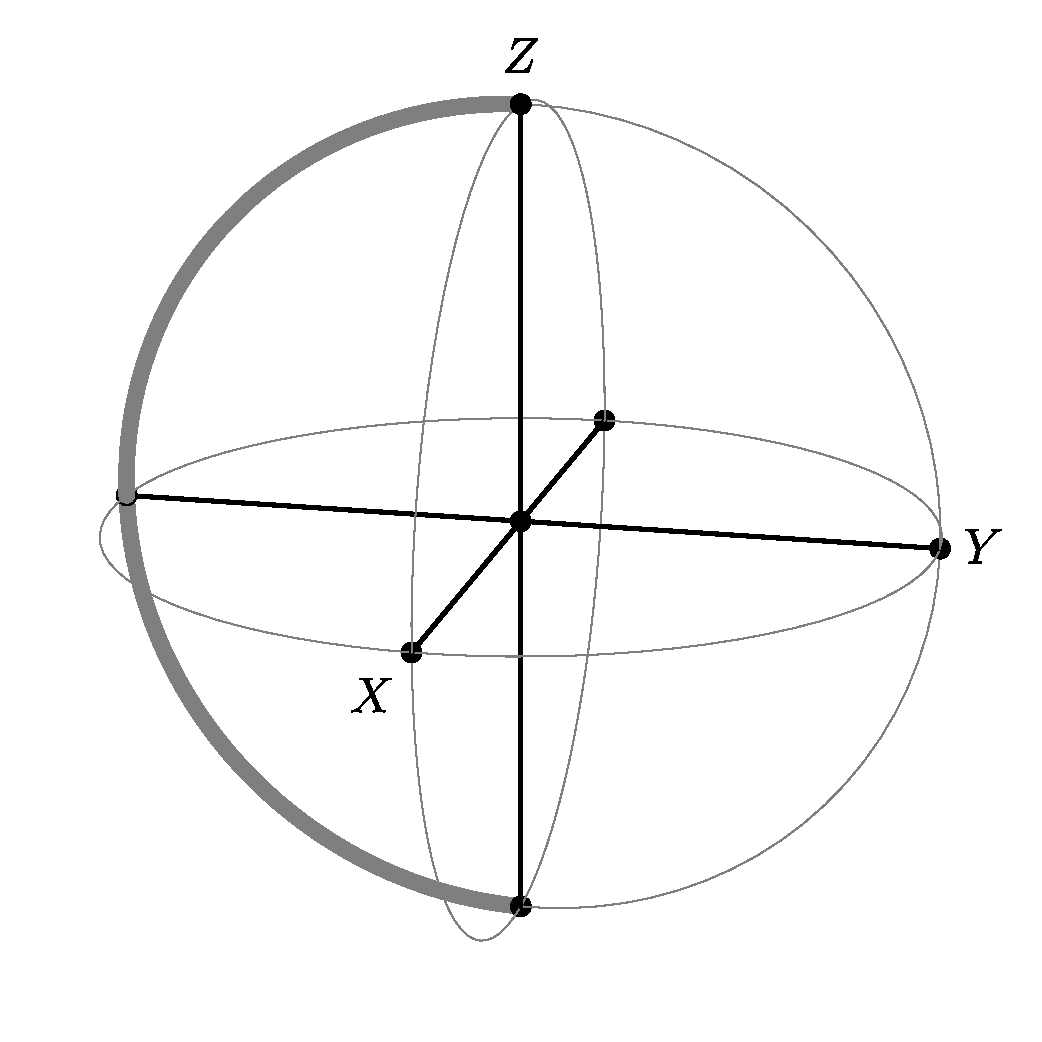
\includegraphics[width=.32\textwidth]{img/blochgate_quench_vec.pdf} &
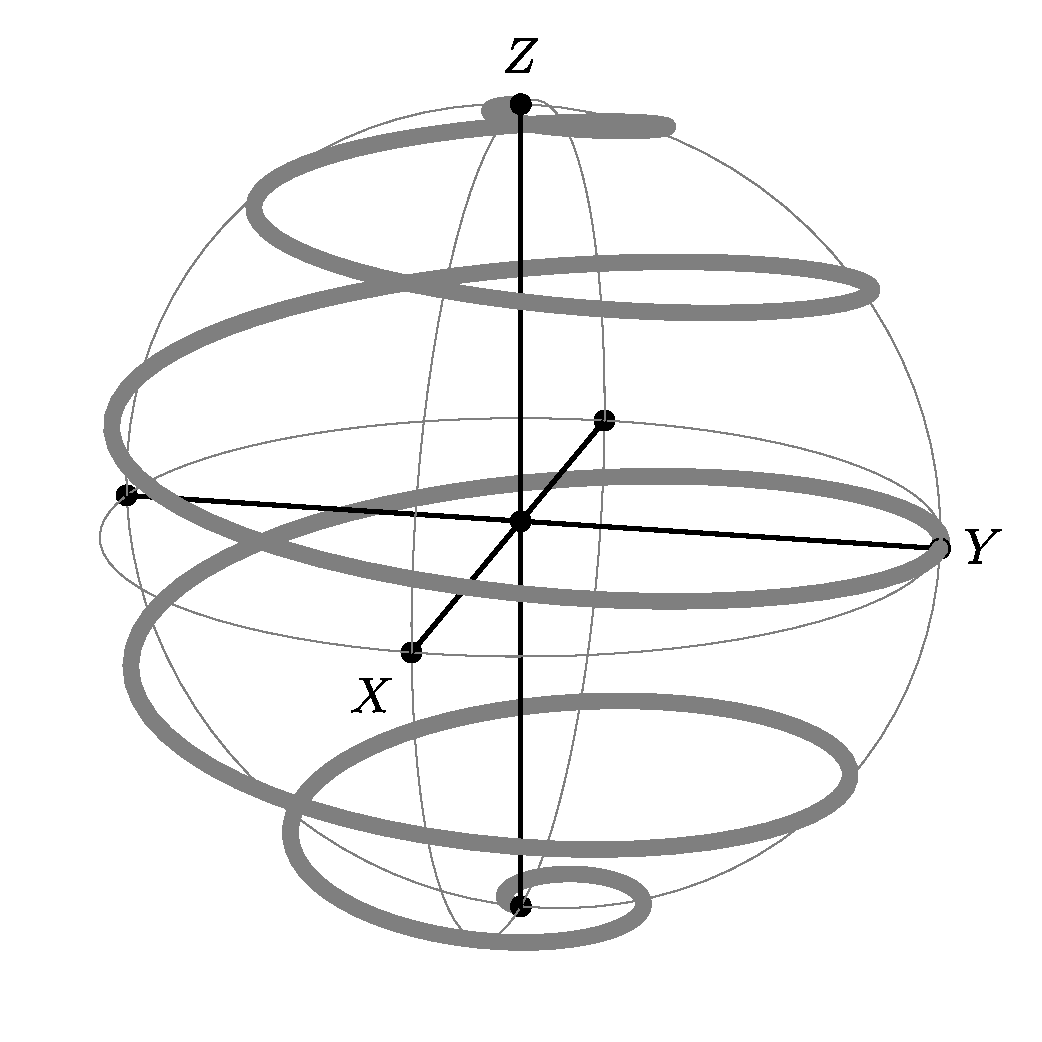
\includegraphics[width=.32\textwidth]{img/blochgate_res_vec.pdf}  	& 
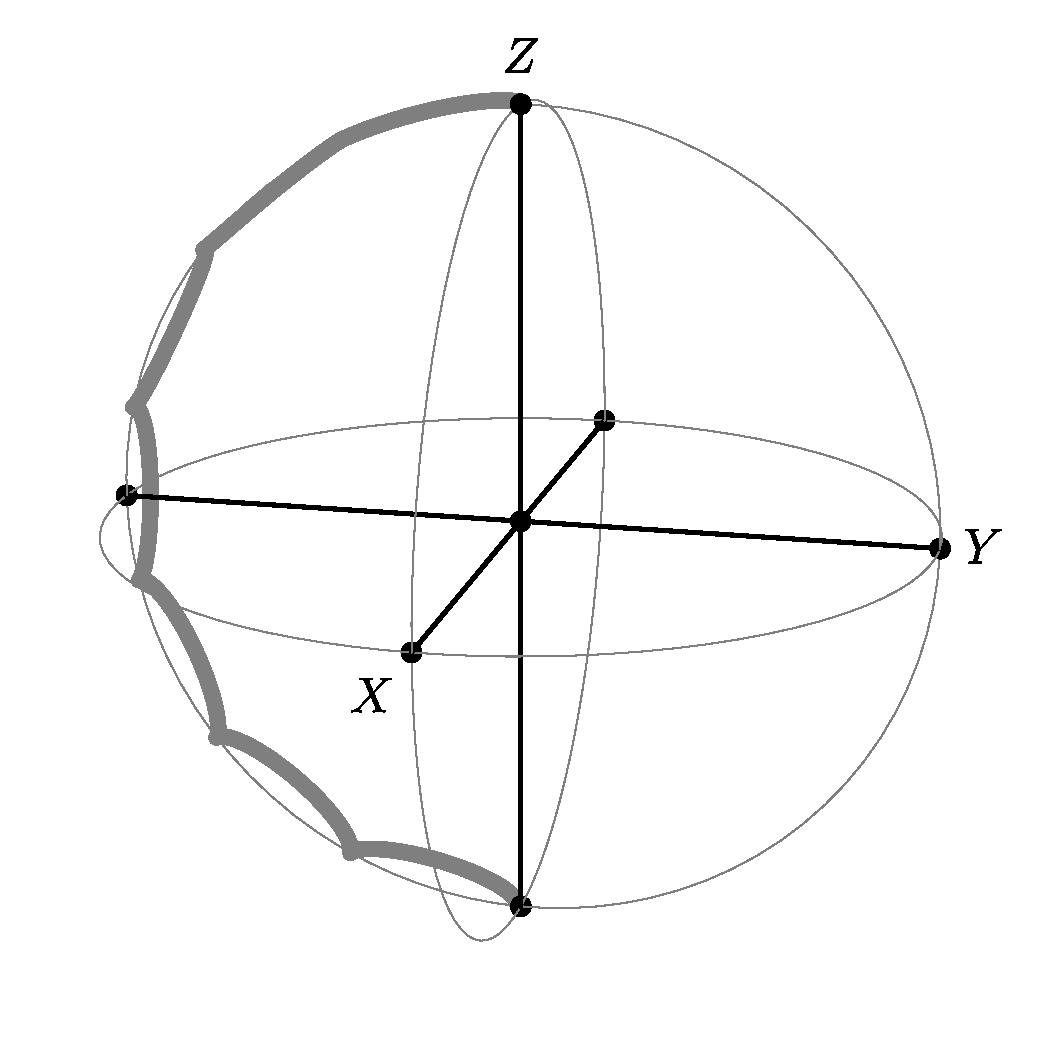
\includegraphics[width=.32\textwidth]{img/blochgate_adiab_vec.pdf}	
\end{tabular}
\caption{The evolution of an initial state $\ket{0}$ by each of the three protocols we discuss, depicted on the Bloch sphere. From left to right: a quench by $H=\Omega X$, a resonant driving protocol (in the lab frame), and an adiabatic protocol executed sufficiently fast, so that some diabatic error is visible ($\Omega T = 7 \pi$). }
\label{fig:xgate_blochsphere}
\end{figure}


\subsection{Resonant driving, and the rotating frame}
\label{sec:resonantdriving}

%
\newcommand{\omd}{ \omega_\text{drive} } 
\newcommand{\omrf}{ \omega_\text{rf} }


Now, let us make the control problem slightly harder, by assuming that the qubit is placed in a magnetic field in the $z$-direction, which we cannot get rid of. We thus supplement the previous problem with the assumptions
\begin{align}
H_\text{bg} &= \frac{ \Delta }{2} Z \quad \text{and} \quad
f_z(t) = 0. \nonumber
\end{align}
In this case, the previous strategy of turning on the field $\Omega X$ causes a rotation around $\vec{n} = ( \Omega, 0, \frac{\Delta}{2} )^T$, which is not what we want. Intuitively, the $Z$ term causes a state to rotate around the equator of the Bloch sphere, whereas the $X$ field pulls the state north at one side of the sphere, and south on the other. If the $Z$-rotations are sufficiently fast, then the movement to the north and south effectively cancel, such that the $X$-gate is never achieved. 

In general, to bridge an eigenvalue gap of size $\Delta$ (note the factor $2$ due to the eigenvalue gap of $Z$), one needs to create a driving field with precisely this amount of energy. We claim that the following Hamiltonian does a better job:
\begin{align}
H(t) &= \frac{\Delta}{2} Z + \A \Big[  \cos(\omd t + \phi) X + \sin(\omd t + \phi) Y    \Big]
\label{eq:Htls_XYdriving} \\
&= \begin{pmatrix}
\frac{\Delta}{2} & \A e^{-i ( \omd t + \phi) } \\
\A e^{ +i (\omd t + \phi) } & - \frac{\Delta}{2}
\end{pmatrix}, \nonumber
\end{align}
%
with $\omd = \Delta$.
Now, when the state oscillates around the equator, the rotation axis $\cos(\omd t) X + \sin(\omd t) Y$ rotates at the same angular velocity, causing it to stay orthogonal to it. This way, it pushes the state north (or south) at all times, without any cancellation effects. 

We make this precise using a smarter perspective, the \textbf{rotating frame} or \textbf{interaction picture}. Effectively, we perceive the system through a camera that looks at the Block sphere, facing downwards from the positive $z$-axis. By rotating the camera at the same angular velocity $\omd$, it seems as if both the rotating state and the rotation axis $\cos(\omd t) X + \sin(\omd t) Y$ stand still, such that we retrieve the quench of \cref{sec:quench}. 

\paragraph{The rotating frame} In general, for any Hamiltonian $H$, we can remove some part $H_0$ from the Hamiltonian, at the cost of making the remaining parts more complicated.  We define the time-dependent basis transformation 
\begin{align}
U_\text{rf}(t) = \exp(+i H_0 t).
\end{align}
We use dots over symbols to denote time derivatives, and let tildes denote quantities in the rotating frame, such that $\tilde{\ket{k}} = U_\text{rf} \ket{k}$.
Importantly, the rotating frame evolves under a different Hamiltonian $\tilde{H}$, which is not quite simply $U_\text{rf} H U_\text{rf}^\dagger$. We derive it by starting from the state $\tilde{\ket{k}}$ and rewriting it using all known rules from the normal frame:
\begin{align*}
i \partial_t \tilde{\ket{k}} &=  i \dot{U}_\text{rf} \ket{k} + i U_\text{rf} \dot{\ket{k}} && \text{Chain rule} \\
&= - H_0 U_\text{rf}(t) \ket{k} + U_\text{rf}(t) H \ket{k} && \text{Applied Sch\"{o}dinger in standard picture}  \\
&= - H_0 \tilde{\ket{k}} +  U_\text{rf} H U^\dagger_\text{rf} \tilde{\ket{k}} && \text{Convert } \ket{j} \text{ back to rotating frame}
\end{align*}
We conclude that the Hamiltonian that governs the rotating frame is given by 
\begin{align}
\tilde{H} = U_\text{rf} H  U^\dagger_\text{rf} - H_0. 
\end{align}
The time-evolution in the rotating frame may be easier to solve. For example, one might obtain the time evolution $\tilde{U}_{t}$ between times $0$ and $t$. The corresponding unitary in the lab frame is then given by %
\begin{align}
U_{t} = U_\text{rf}^\dagger(t) \tilde{U}_{t}.
\label{eq:labframe}
\end{align}
To gain some more intuition for the effect of the rotating frame: on a Hamiltonian $H$ with matrix elements $H_{jk}$, the basis transformation $U = e^{i \delta \ket{\ell}\bra{\ell} t}$ causes the $\ell$'th row and column obtain a rotating phase: 
%
\begin{align*}
%
%
%
%
%
%
%
%
\tilde{H} = 
\begin{pmatrix}
H_{11} & \dots & H_{1 \ell} e^{-i\delta t} & \dots & H_{1n} \\
\vdots &  \ddots &   \vdots &     & \vdots \\
H_{1 \ell}^* e^{i\delta t} & \dots & H_{\ell \ell} -\delta & \dots &H_{ \ell n} e^{i\delta t} \\
\vdots & 		&  \vdots & \ddots	& \vdots	\\
H_{1n}^* & \dots & H_{\ell n}^*  e^{-i\delta t} & \dots & H_{nn}  
\end{pmatrix}
\end{align*}

\paragraph{Rabi cycles} Turning back to our rotation on the Bloch sphere, we can remove the compulsory magnetic field $H_\text{bg}$ through the basis transformation $U_\text{rf} = \exp(+i \frac{\omega_\text{rf}}{2} Z)$. The rotating version of the Hamiltonian in \cref{eq:Htls_XYdriving} then becomes 
%
\begin{align}
\tilde{H} &= \left( \frac{\Delta - \omega_\text{rf}}{2} \right) Z  + \Omega U_\text{rf} \Big[ e^{- i ( \omd t + \phi ) } \sigma^+ + e^{+ i ( \omd t + \phi )} \sigma^- \Big] U_\text{rf}^\dagger   \label{eq:TLSinRF} \\
	&= \left( \frac{\Delta - \omega_\text{rf}}{2} \right) Z + \Omega \Big[ 
	e^{-i (\omega_\text{drive} - \omega_\text{rf} ) t - i \phi  } \sigma^+ 
	+  e^{+i (\omega_\text{drive} - \omega_\text{rf})t + i \phi } \sigma^- \Big]. \nonumber
\end{align}
In the first step, we used that $\sigma^\pm = \frac{X \mp i Y}{2}$, and in the last step, we used $U_\text{rf} \sigma^\pm U^\dagger_\text{rf} = e^{\pm i \omrf t } \sigma^\pm$. Note the difference between the omega's: $\omd$ is a physical thing, describing the oscillation frequency of the $X$ and $Y$ fields in the lab frame, whereas $\omrf$ is just a parameter invented by us: it describes how fast our camera is rotating. In particular, we like to choose $\omrf = \omd$, so the camera follows the driving axis, making the Hamiltonian time-independent: 
%
\begin{align}
\tilde{H} &= \left( \frac{\Delta - \omd}{2} \right) Z + \Omega \Big[ 
	e^{- i \phi  } \sigma^+ 
	+  e^{+ i \phi } \sigma^- \Big]    \\
	&= \begin{pmatrix}
\delta / 2 & \A e^{-i \phi} \\
\A e^{+i \phi} & -\delta / 2
\end{pmatrix}. \nonumber
\end{align}
In the last step, we defined the \textbf{detuning} or \textbf{off-resonance} $\delta = \Delta - \omd$. Evolution by $\tilde{H}$ dictates \emph{Rabi flopping}:
\begin{align}
\tilde{U}_t = e^{-i \tilde{H} t } = \cos( n t ) \mathds{1} - i \sin( n t ) \left( \frac{ \vec{n} }{n} \right) \cdot \vec{\sigma}  \label{eqn:Udrive} \\
\text{with } \vec{n} = \begin{pmatrix} \cos(\phi) \A \\ \sin(\phi) \A \\ \delta / 2 \end{pmatrix}, 
\quad n = \sqrt{\A^2 + \frac{\delta^2}{4}}.  \nonumber
\end{align}
From this, we conclude that a perfect rotation  around the axis $\cos(\phi) X + \sin(\phi) Y$ can be performed if $\delta=0$ and $t =\frac{\pi}{2\A}$, meaning that each computational basis state is inverted into the other. Specifically, at $\phi=0$, we retrieve the $X$-gate, and at $\phi = \pi/2$ the gate $Y$. Remember that all of this is in the rotating frame -  we should not forget to move back to the lab frame using \cref{eq:labframe}, which re-inserts the accumulated phase due to $H_\text{bg}$. We will use the term \textbf{resonant driving} to indicate the choice $\delta=0$ with the aim to implement such transitions between computational basis states.  



We also consider what happens whenever the driving is \textbf{off-resonant}, in the limit where $|\delta| \gg |\A|$. Here, $\vec{n}$ points mainly in the $Z$-direction, causing hardly any mixing of the computational basis states, but rather giving the states a hard-to-predict relative phase. This effect is otherwise known as the Autler-Townes or AC Stark effect. %

\paragraph{The rotating wave approximation}
Sometimes, it may be impossible to have both the $X$ and $Y$ fields on at the same time in \cref{eq:Htls_XYdriving}. In that case, we may still work with a Hamiltonian of the form 
\begin{align}
H(t) &= \frac{\Delta}{2} Z + 2 \A   \cos(\omd t + \phi) X  
\label{eq:Htls_Xdriving} \\
&= \begin{pmatrix}
\frac{\Delta}{2} & \A \left( e^{-i ( \omd t + \phi) } + e^{+i ( \omd t + \phi) } \right) \\
\A  \left( e^{-i ( \omd t + \phi) } + e^{+i ( \omd t + \phi) } \right)  & - \frac{\Delta}{2}
\end{pmatrix}, \nonumber
\end{align}
(note that we changed $\Omega \rightarrow 2 \Omega$ here), which looks slightly more daunting in the same rotating frame we used before: 
\begin{align*}
\tilde{H} = & \left( \frac{\Delta - \omega_\text{rf}}{2} \right) Z \\ 
& + \Omega \Big[ 
	\sigma^+ \left( e^{-i (\omega_\text{drive} - \omega_\text{rf} ) t - i \phi  }
					+ e^{+i (\omega_\text{drive} + \omega_\text{rf} ) t + i \phi  } \right) \\
& \hphantom{ + \Omega  }
  + \sigma^- \left( e^{-i (\omega_\text{drive} + \omega_\text{rf} ) t - i \phi  }
					+ e^{+i (\omega_\text{drive} - \omega_\text{rf} ) t + i \phi  } \right) \Big] \\
\end{align*}
%
%
An important clean-up step that is canonically taken at this point is the \textbf{rotating wave approximation} (RWA). It tells us that $\omega_\text{rf} - \omega_\text{drive}$ is a fairly small number, whereas $\omega_\text{rf} + \omega_\text{drive}$ is huge compared to typical time-scales in our problem. Therefore, the terms $e^{\pm i (\omega_\text{rf} + \omega_\text{drive})}$ keep causing \emph{off-resonant} rotations back and forth, so fast and so tiny that they merely cause a state to wiggle in phase space, without changing the qualitative behavior of the system. The RWA tells us that we can remove these terms from the Hamiltonian. 
This approximation is only valid whenever \cite{Irish2005}
\begin{align*} %
| \omega_\text{drive} - \omrf | \ll& \omrf, \omega_\text{drive}  && \text{ such that the other exponentials do rotate slowly, and } \\  
 	\Omega \ll& \omrf, \omega_\text{drive} && \text{ such that the wiggles are small.}
\end{align*}
%
One can check that discarding these quickly oscillating terms leaves us with the same Hamiltonian we found in \cref{eq:TLSinRF}, and all the previous conclusions about (off-)resonance apply again. 

\paragraph{The resonant $X$-gate} Turning back to our $X$-gate: the gate can be obtained using the Hamiltonians in \cref{eq:Htls_XYdriving} or \cref{eq:Htls_Xdriving}. In \cref{fig:xgate_blochsphere}, we sketch the trajectory that an initial state $\ket{0}$ follows on the Bloch sphere in the \emph{lab frame}, in which it quickly oscillates while descending down the sphere. For the case in which driving only occurs along the $X$-axis (\cref{eq:Htls_Xdriving}), we sketch the same time evolution in the \emph{rotating frame} in \cref{fig:xgate_rwa}, such that the error due to the quickly rotating waves is visible. 


\begin{figure}
\centering
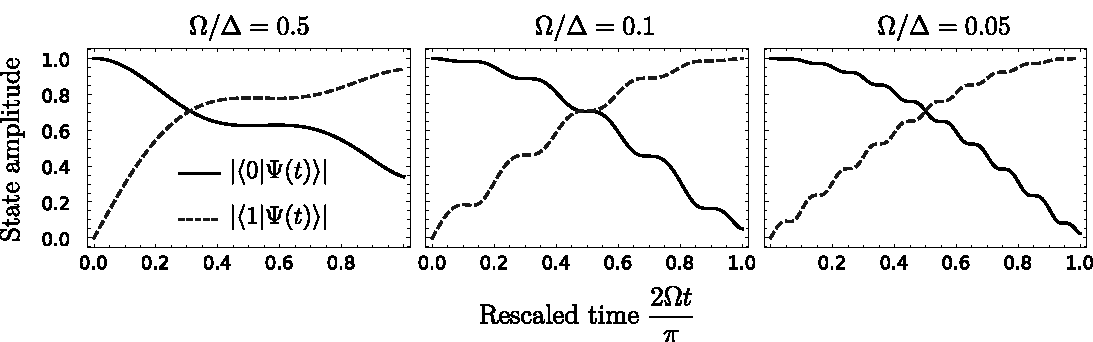
\includegraphics[width=.95\textwidth]{img/DriveRWAPlots_row} 
\caption{The evolution of the initial state $\ket{\Psi(0)} = \ket{0}$ due to the Hamiltonian in \cref{eq:Htls_Xdriving},  in the rotating frame. We assume resonance ($\omrf = \omd = \Delta$). When $\Omega / \Delta$ is \emph{small}, as on the right-hand side, then the RWA is justified, and the evolution is very similar to the quench $H = \Omega X$. When $\Omega / \Delta = 0.1$, the approximation errors are much more visible, and when $\Omega / \Delta = 0.5$, the evolution is far from the aimed trajectory. }
\label{fig:xgate_rwa}
\end{figure}


\paragraph{} In \cref{sec:resdrive}, we will come back to the toy model presented here, as it turns out to also be relevant when constructing a quantum gate that acts on multiple qubits. 


\subsection{Adiabatic passage}
\label{sec:adiabatic}
Assume you are asked to transport a tray filled with fancy-looking yet somewhat wobbly cocktails. Clearly, you want the tray to arrive at its destination in the same \emph{state} that it is now. Your best approach is to accelerate the tray rather slowly, or else you may spill the drinks! 

The same line of thought turns out to hold in quantum mechanics. If at $t=0$ a system is in the $j$th eigenstate of $H(t)$, then it will still be approximately in the $j$th eigenstate at later times, provided that $j$ is non-degenerate and $H(t)$ changes sufficiently slowly. Note that the \emph{eigenstates} themselves have probably changed in time, providing us with an intuitive method to change a quantum state to our liking. We will study the precise mechanics behind the \textbf{adiabatic theorem}, following David Griffiths \cite{Griffiths2005}. 

As $H(t)$ is now time-dependent, we define that \textbf{instantaneous eigensystem} of $H$ as the eigenvalues $\lambda_j(t)$ and eigenvectors $\ket{\psi_j(t)}$ at time $t$:\footnote{Note that there is an ambiguity in the \emph{phase} of the eigenvectors, which can be adjusted at each time $t$. We do not define these phases as these turn out to be unimportant for our purposes, but a rigorous approach can be found in Ref. \cite{Born1928}.}
\begin{align}
H(t) \ket{\psi_j(t)} = \lambda_j(t) \ket{\psi_j(t)}.
\label{eq:adiabatic_evec}
\end{align}
We can express any solution to Schr\"{o}dinger's equation $\ket{\Psi(t)}$ in the basis of instantaneous eigenstates,
\begin{align}
\ket{\Psi(t)} = \sum_j c_j(t) e^{-i \theta_j(t)} \ket{\psi_j(t)},  \label{eq:adiabaticSolution} \\
\theta_j(t)  = \int_{s=0}^{t} \lambda_j(s) ds', \nonumber
\end{align}
where $\theta_j(t)$ is a dynamical phase that we take out of $c_j(t)$ for later convenience. Plugging this into SE, and omitting explicit time-dependence for readability, we obtain
\begin{align}
\sum_j \left( \dot{c}_j \ket{\psi_j}  + c_j \partial_t \ket{\psi_j} - i c_j \dot{\theta_j} \ket{\psi_j} \right) e^{-i \theta_j} &= \sum_j c_j \lambda_j e^{-i \theta_j} \ket{\psi_j} \nonumber \\
\sum_j \left( \dot{c}_j e^{-i \theta_j}  \ket{\psi_j} + c_j e^{-i \theta_j} \partial_t \ket{\psi_j} \right) &= 0 \nonumber \\
\dot{c}_k e^{-i \theta_k} + \sum_j c_j  e^{-i \theta_j} \bra{\psi_k} \partial_t \ket{\psi_j} &= 0 \nonumber \\
\dot{c}_{k}(t) &= -\sum_j c_j   \bra{\psi_k} \partial_t \ket{\psi_j}  e^{-i ( \theta_j - \theta_k ) }.
\label{eqn:adiabatic_ck}
\end{align}
In the first step, we canceled the last two terms, and in the second, we took the projection to the $k$'th eigenvector. The quantity $\bra{\psi_k} \partial_t \ket{\psi_j}$ already gives some insight in what we mean with the adiabatic theorem: if the instantaneous eigenvector $\ket{\psi_j(t)}$ rotates in the direction of \emph{other} eigenvectors very slowly, then the amplitudes $c_k(t)$ of other eigenvectors do not change too much. To better quantify how much this `leakage' to other states actually is, we need to replace $\bra{\psi_k} \partial_t \ket{\psi_j}$ by something that we obtain as follows, by differentiating the eigenvalue equation, \cref{eq:adiabatic_evec}:
\begin{align*}
\dot{H} \ket{\psi_j} + H \partial_t \ket{\psi_j} &= \dot{\lambda}_j \ket{\psi_j} + \lambda_j \partial_t \ket{\psi_j} \\
\bra{\psi_k} \dot{H} \ket{\psi_j} + \bra{\psi_k} H \partial_t \ket{\psi_j} &= \dot{\lambda}_j \braket{\psi_k}{\psi_j} + \lambda_j \bra{\psi_k} \partial_t \ket{\psi_j}. 
\end{align*}
Hence for the `leaky' states $k \neq j$,
\begin{align*}
\bra{\psi_k} \dot{H} \ket{\psi_j} + \lambda_k \bra{\psi_k} \partial_t \ket{\psi_j} &= \lambda_j \bra{\psi_k} \partial_t \ket{\psi_j} \\
\bra{\psi_k} \partial_t \ket{\psi_j} &= \frac{ \bra{\psi_k} \dot{H} \ket{\psi_j} }{ \lambda_j - \lambda_k }.
\end{align*}
Note that in this step, we had to assume that $\lambda_j$ is \emph{non-degenerate}. Plugging this back in to \cref{eqn:adiabatic_ck}, 
\begin{align}
\dot{c}_k(t) = - c_k \bra{\psi_k} \partial_t \ket{\psi_k} - \sum_{j \neq k} \frac{ \bra{\psi_k} \dot{H} \ket{\psi_j} }{ \lambda_j - \lambda_k } e^{-i (\theta_j - \theta_k )}.
\label{eqn:adiabatic_ck2}
\end{align}
Now, this expression is \emph{exact}. The adiabatic approximation asserts that the oscillations $e^{-i (\theta_j - \theta_k )}$ are so fast compared to other timescales in our system that on average the second term does not influence $\dot{c}_k(t)$.  The rigorous proof was first given by Born and Fock \cite{Born1928}, but we follow the more accessible notation of Ref. \cite{Katanaev2011}.

Firstly, we should define what we mean with `slow'. Let $\tilde{H}(s)$ be a Hamiltonian on the rescaled time interval $s \in [0,1]$.
%
Then, we can compare the same quantum protocol at different time scales: for each value of total time $T$, we define the time-dependent Hamiltonian $H_T(t) = \tilde{H}(t/T)$. 

Now, assume the system is, at $t=0$, initialized in the $\ell$th eigenstate $\ket{\Psi(0)} = \ket{\psi_\ell(0)}$. In other words, we start with state amplitudes $c_k(t=0) = \delta_{k \ell}$. Moreover, we assume that for all $t$ and for all $k \neq \ell$, the energy gap $|\lambda_j(t) - \lambda_k(t)|$ is bounded from below by $\Delta$. Then, under evolution by $H_T(t)$ \cite{Katanaev2011},
\begin{align}
1 - | \braket{\Psi(T)}{\psi_\ell(T) } |^2 = O\left( \frac{1}{ \Delta^2 T^2} \right)  .
\label{eq:adiabaticthm}
\end{align}
In other words, the system's state $\ket{\Psi(t)}$ remains close to the instantaneous eigenstate $\ket{\psi_\ell(t)}$, as long as the total time $T$ of the evolution is sufficiently large, implying slow changes to $H(t)$. Likewise, by conservation of probability, all other states must be minimally populated: $c_k = O\left( \frac{1}{ \Delta^2 T^2} \right)  $ for all $k \neq \ell$. 

Ref. \cite{Katanaev2011} technically assumes a finite-dimensional system, and that the degeneracies of eigenvalues stay constant (i.e. no crossings of energy levels are allowed), even for states other than our initial state $\ket{\psi_\ell(0)}$. The scaling itself is tight, in the sense that examples with the scaling stated in \cref{eq:adiabaticthm} exist, so the bound cannot be improved. 


%
%
%
%
%
%
%
%
%
%
%
%

\begin{figure}
\centering
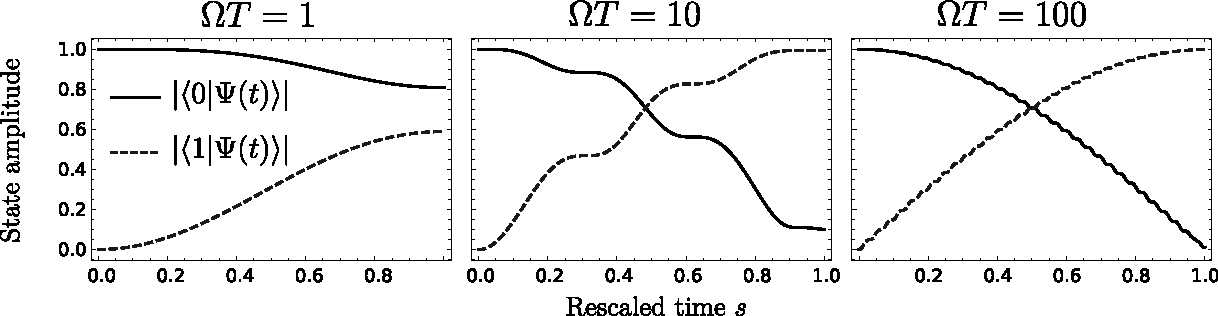
\includegraphics[width=.95\textwidth]{img/AdiabaticPlotsStacked.pdf} 
\caption{The state amplitudes $|c_k(t)|$ during the adiabatic protocol in \cref{eq:xgate_adiabatic}, for different total times $T$. The initial state is always $\ket{\Psi(0)} = \ket{0}$. When $\Omega T \gg 1$, the system closely follows the corresponding instantaneous eigenstate, up to tiny oscillations. When $\Omega T = 10$, the errors are much more visible, and at $\Omega T = 1$, the system's state cannot keep up with the quickly changing Hamiltonian anymore. The evolution is then very different from the aimed $X$-gate.  }
\label{fig:adiabatic_timescales}
\end{figure}


\paragraph{The adiabatic $X$-gate}
Let us turn back to the control task of performing the gate $U_t = X$, as defined in \cref{eq:controlproblem}. Remember the quench of $H=\Omega X$ in \cref{sec:quench}, which rotates an initial state $\ket{0}$ first towards the negative $Y$-axis, and then further down towards $\ket{1}$ at the negative $Z$-axis. Similarly, the state $\ket{1}$ is rotated towards $+Y$ and then towards $+Z$. We can simulate that evolution in the adiabatic limit, using 
\begin{align}
H_T(t) = \Omega \left[ \cos \left( \frac{\pi t}{2 T}  \right) Z - \sin \left( \frac{\pi t}{2 T}  \right) Y \right].
\label{eq:xgate_adiabatic}
\end{align}
One can check that there are no eigenvalue crossings, and in fact, the energies remain constant at $\pm \Omega$ for each $t$. Thus, $\Delta = 2 \Omega$ in this case. By choosing $\Omega T$ sufficiently large, can make sure that an initial state $\ket{0}$ or $\ket{1}$ follows the trajectory defined by the quench to arbitrary accuracy. To obtain a proper $X$-gate, one also has to care about the accumulated dynamical phases, which equal $e^{\pm i \Omega T}$ in each case. These phases become equal\footnote{Note that whenever $\Omega T$ is odd, a dynamical phase of $-1$ is given to each of the basis states. In our setting, this is an irrelevant global phase, but note that there exist settings in which a more careful treatment of phases is required.}
 again whenever $\Omega T \in \mathbb{Z}$. The evolution due to \cref{eq:xgate_adiabatic} is plotted on the right in \cref{fig:xgate_blochsphere}. We chose $\Omega T = 7 \pi$, which is sufficiently small that typical \emph{diabatic} errors are visible. The influence of errors at various time scales is compared in \cref{fig:adiabatic_timescales}.



%



\paragraph{}
In \cref{part:adiabatic}, we will consider precisely the waiter's task to transport a tray of cocktails, where now the cocktails happen to be quantum states that we aim to transport over a graph. Again, we will find that, for sufficiently slow changes to $H$, the state can be transported with arbitrary accuracy, provided that there is a \emph{gap} $\Delta$ at all times. 





\section{How to transport a quantum state}
\label{sec:howtotransport}
In the world of \emph{classical} computers, we can hardly imagine living without extensive communication between our devices - whether it is over the internet, a USB cable or bluetooth. Similarly, a future \emph{quantum} computer is expected to require communication with other quantum devices, as is also stated as one of DiVincenzo's criteria \cite{DiVincenzo2000}. Here, one should not only think of some quantum internet that connects individual users, but also of short-distance communication between nearby quantum processors: these may be limited in physical size, but can be entangled to collectively perform a larger calculations \cite{Vandersypen2017,Brown2016}. This section reviews the most important known results from the art of moving a quantum state from one place to another. 

\paragraph{}
The no-cloning theorem complicates communication of quantum states: it is impossible to make several copies and perform various attempts of lossy communication. Luckily, there are various tricks to boost fidelities, such as transferring error-correcting codes, or using quantum repeaters. A network of repeaters could work as follows. The noisy communication channel allows a set of parties to distribute entangled Bell pairs among each other, which can be turned into high-fidelity Bell states using entanglement distillation \cite{Bennett1996,Bennett1996a,Kalb2017}. Next, using entanglement swapping and teleportation, arbitrary qubits can be sent with high fidelity \cite{Wehner2018}. Transporting states and establishing entanglement appear to be closely related, and we will encounter many physical systems where both go hand in hand.

When it comes to communication over larger distances, photons are a clear winner. They can encode quantum states in various ways (e.g. polarization, Fock number, spatial modes, time-bins), and can travel at high speeds through vacuum or optical fibers. Moreover, high-quality optical fiber networks are already widely implemented for classical communication applications. There is ongoing research on conversion between photonic states and various other qubit platforms, such as trapped ions \cite{Monroe2014}, superconducting qubits \cite{Soltani2017}, cold atoms \cite{Bechler2018,Tiarks2019}, NV centers \cite{Dreau2018}, or general qubits locked in a cavity \cite{Vogell2017}. 

For shorter distances, the conversion to light may be omitted in favor of other techniques, which is the focus of the remainder of this chapter and, in particular, of \cref{part:adiabatic} of this thesis. Some types of qubits are mobile by nature, and can be physically displaced. Examples are electrons or atoms that are held in some artificial potential field, such that they can tunnel between nearby minima of the potential.
%
Other information carriers are immobile, such as atoms in a crystal or in a molecule, and one can picture information `flowing' through the system while the qubits themselves sit still. The latter form of communication can intuitively be compared to flicking a rope that is spanned between two users: the resulting wave travels a long distance between the ends of the rope, while the rope's constituents merely move within their locally confined space. In this sense, classical communication of electrical signals over a copper wire is not that much different. In the following, we focus on both mobile and immobile qubits, as long as the locations of the qubits can be modeled as a finite and discrete graph-like structure. 

\paragraph{}
Having set our domain of interest, we may now ask the question \emph{for which models can we transfer quantum information between Alice and Bob, using which controls?} This brings together the topics of condensed matter models and quantum control: we assume a system defined by an interaction type and a graph, such as discussed in \cref{sec:cmtmodels}, where two vertices of the graph are marked as Alice (a) and Bob (b). Then, similar to \cref{sec:manipulate}, we tweak the system parameters in such a way that the unitary time evolution $U_T$ after some time $T$ is such that Bob can infer what the initial state at Alice was. 


As a warning to the reader, many transfer protocols will look very similar. To distinguish the subtle differences between various theoretical proposals of state transfer, it is important to consider the precise \emph{model} (including the type of particles and type of interaction), the \emph{graphs} on which the transfer works, the \emph{controls} (typically a quench or adiabatic passage), and the assumed \emph{initial state} of the system. 
Important figures of merit used for comparison are mainly the (theoretical) transfer speed and fidelity, but also include the feasibility of the \emph{control requirements}, such as the number of controllable parameters in the Hamiltonian. 

An overview of the protocols we discuss here is given in \cref{tab:transfer}, and more elaborate overviews can be found in Refs. \cite{Bose2007,Nikolopoulos2014,Menchon-Enrich2016}. We choose to categorize the transfer protocols based on the \emph{initial state}, namely whether they start with a \emph{single} (or a small number of) excitation, or with a number that is \emph{very large} (i.e. growing with the system size $N$). Within these groups, we distinguish whether the protocol is based on a quench or adiabatic evolution.

One important transfer approach that does not fit within our categorization is the use of sequential \texttt{SWAP}-like gates, which are less interesting from a condensed matter viewpoint. Also not discussed are topological variants, such as Thouless pumps \cite{Thouless1983,Voorden2019}, which are typically concerned with effective charge transfer or displacement of a particle's center of mass, rather than communicating quantum information \cite{Citro2016}. Note that the repeated nature of topological pumps, which displace a quantum amplitude by a certain number of sites per iteration, is somewhat similar to sequence of swaps from a quantum control perspective. 





%

\setlength{\tabcolsep}{.2cm}
\begin{table}
\begin{center}
\begin{tabular}{c|c|c}
%
 &
\begin{minipage}{4.5cm} \begin{center}
 \textbf{Single excitation} 
 \begin{align*}
	H =  \sum W_{jk}  {j} {k}
 \end{align*} \vspace{-1cm}
 \begin{align*}
 \ket{\Psi(0)} =  \ket{a}
 \end{align*} \vspace{-1cm}
 \begin{align*}
\text{dim}(\mathcal{H}) \sim N
 \end{align*} \vspace{-.5cm}
\end{center} \end{minipage}
 &  
 \begin{minipage}{4.2cm} \begin{center}
 \textbf{Half filling}
 \begin{align*}
 H = \sum w_{jk} h_{jk}
 \end{align*} \vspace{-1cm}
 \begin{align*}
  \ket{\Psi(0)} =  \ket{\phi}_a \otimes  \ket{\text{rest}}
  \end{align*} \vspace{-1cm}
 \begin{align*}
 \text{dim}(\mathcal{H}) \sim \exp(N) 
 \end{align*} \vspace{-.5cm}
\end{center} \end{minipage}

\\ \hline 
\begin{minipage}{4.5cm} \begin{center}
	\mbox{} \\
	\textbf{Quench}
	\flushleft{ \begin{itemize}
	\item Fast
	\item Passive couplings
	\item Accurate controls required
	\end{itemize} } 
	\mbox{} \\
\end{center} \end{minipage}

&  
\begin{minipage}{4.5cm} \begin{center}
(near-)perfect  \\ state transfer	
\end{center} \end{minipage}
& 
\begin{minipage}{4.2cm} \begin{center}
XXX with straddling, \\  mirror inverting chains
\end{center} \end{minipage}
\\ \hline
\begin{minipage}{4.2cm} \begin{center}
\mbox{ } \\
\textbf{Adiabatic}
\flushleft{
	\begin{itemize}
	\item Slow
	\item Time-dependent couplings
	\item Resilient to control errors
	\end{itemize}
}
\mbox{} \\
\end{center} \end{minipage}
 & 
\begin{minipage}{4.5cm} \begin{center}
 STIRAP, CTAP, \\ and dark passage \\ (\cref{chap:ctap})
\end{center} \end{minipage}
  & 
\begin{minipage}{4.2cm} \begin{center}
XXX model \\ (\cref{chap:heisenberg})
\end{center} \end{minipage}

\\ \hline

\end{tabular}
\end{center}
\caption{An overview the state transfer protocols we consider.}
\label{tab:transfer}
\end{table}


%
%
%
%
%
%
%
%
%
%
%
%
%
%
%
%
%
%
%
%
%
%
%
%
%
%
%
%
%
%
%
%
%
%
%
%
%
%
%
%
%
%
%
%
%
%
%
%
%
%
%
%
%
%

%


\subsection{Single excitation hopping}
\label{sec:transfer_single_exc}
As far as the models are concerned, it turns out that some physical systems lead to the same mathematics. The ferromagnetic XX and XXX models, with as local entities qubits, are typically taken to be in a magnetic field of the form $H = -B \sum_j Z_j$, such that $\ket{0^N}$ is the ground state. From that state, Alice can locally initialize 
\begin{align*}
\ket{\Psi(0)} = \alpha \ket{0}_a \otimes \ket{0^{N-1}}_\text{rest} + \beta \ket{1}_a \otimes \ket{0^{N-1}}_\text{rest}.
\end{align*}
The initial term is an eigenstate that will not evolve, whereas the second term will follow some evolution through the $N$-dimensional space of states with Hamming weight $1$. We may use the notation $\ket{ \{j\} } =  X_j \ket{0^N}$ to denote the state with all qubits in the state $0$, except for qubit $j$ which is in state $1$. If there is no ambiguity, we sometimes omit the curly brackets. The Hamiltonian in the sector of a single excitation then reads
\begin{align}
H = \sum_{j, k \in V} W_{jk} \ket{\{j\}} \bra{\{k\}}
\label{eqn:Hpst}
\end{align}
This is also precisely the Hamiltonian that describes a single quantum particle (such as a fermion or boson) that hops over a graph: these are described by the interaction $\sum w_{jk} f^\dagger_j f_k$ (plus potential two-body terms that are now irrelevant), together with the translation $\ket{\{j}\} = f^\dagger_j \ket{0}$. Hence, any protocol that assumes \cref{eqn:Hpst} may represent either of the three models, and we collectively describe them as \emph{single excitation hopping}. The main differences between the models are:
\begin{itemize}
\item for both the free particle hopping and the XX model, with hopping amplitudes or coupling strengths $w_{jk}$, the matrix $W$ is precisely the adjacency matrix of the graph: $W = w = A_G$
\item for the XXX model, with couplings $w_{jk}$, the matrix $W$ is the Laplacian $L_G$ of the graph: $W = L_G = D_G - A_G$, where $D_G$ is the diagonal matrix with entries corresponding to the degree of each vertex.
\end{itemize}

\paragraph{Quenches} 
When considering quenches, one quickly arrives at the field of \textbf{perfect state transfer} (PST) which attempts to find times $t$ and weight matrices $W$ precisely such that 
\begin{align*}
\bra{ \{ b \} } e^{-i W t} \ket{\{a\}} = 1,
\end{align*}
where $a$ and $b$ denote the locations of Alice and Bob, respectively. This setting is equivalent to setting of \textbf{continuous time quantum walks} \cite{Mulken2011} where $W$ denotes the adjacency matrix of a graph. In 2004, two independent works reported on perfect transfer between the endpoints of an open chain, using the weights 
\begin{align*}
W_{j,j+1} \propto \sqrt{ j (N-j) },  \quad W_{j j} = 0.
\end{align*}
The results were found for very different physical models, namely the XX model \cite{Christandl2004}, and an electron hopping between quantum dots \cite{Nikolopoulos2004}. The configuration is now often called the \textbf{Krawtchouk chain}, and we will encounter it again in \cref{chap:krawtchouk}. The couplings $W$ are precisely such that the dispersion (the energy, as a function of wave number) becomes linear. Here and in the following, we often consider the \textbf{mirror symmetry} of a chain, such that even eigenstates have an eigenvalue $+1$ under the relabeling operation $j \rightarrow N-j+1$, and odd eigenstates have an eigenvalue $-1$. In this case, the energies of the odd eigenstates \emph{interlace} the energies of the even states. Then, for some energy scale of the coupling $W$, the even eigenstates all have \emph{even} eigenvalues, and the odd eigenstates have \emph{odd} eigenvalues. Hence, there is some evolution time, for which
\begin{align*}
\ket{\Psi_\text{even}} \rightarrow e^{-i (2 k) \pi} \ket{\Psi_\text{even}}, \\
\ket{\Psi_\text{odd}} \rightarrow e^{-i (2 k + 1) \pi} \ket{\Psi_\text{odd}}.
\end{align*}
By giving the odd components of \emph{any} state a minus sign, one exactly performs a mirror operation on the state: one does not only obtain PST, but a mirror operation on any single-excitation state. For non-interacting theories, such as free fermions and the XX model, this remains true for sectors with any number of excitations.

Ever since these early results, many more graphs and weight configurations were found to perfectly transfer a state \cite{Kay2010a,Godsil2012}, sometimes even well after they were originally introduced, such as the Polychronakos chain $H_P$ that we address in \cref{chap:pc}. 

The ferromagnetic XXX model, with a single excitation, is very similar to the case of the XX model, except that the Hamiltonian now has diagonal entries. Bose kickstarted the field of state transfer in 2003 \cite{Bose2003}  by observing that, on a uniformly coupled linear chain, an excitation initially at site 1 would appear at site $N$ with high probability after a sufficiently large time. Such cases are sometimes called \textbf{near-perfect state transfer}, and various other examples exist \cite{Godsil2012a,Vinet2012,Banchi2017}.

\paragraph{Adiabatic} 
In adiabatic protocols, we typically assume time-dependent control over the couplings $W_{jk}(t)$ in \cref{eqn:Hpst}. At $t=0$ and $t=T$, the adiabatic eigenstate of the system must be located on Alice's or Bob's subsystem, which generally means that these subsystems are isolated: the couplings $W_{jk}$ connected to Alice or Bob are then $0$. In between, the couplings $W_{jk}$ are engineered to connect aforementioned eigenstates, without causing a degeneracy. A protocol that follows this framework necessarily requires a \emph{counter-intuitive} pulse sequence: the couplings to the \emph{receiver} are initially strongest and are lowered over time, whereas the couplings to the \emph{sender} start at $0$ and grow stronger towards the end of the protocol. A sketch of such a protocol is given in \cref{fig:adiabatic_protocol_sketch}. 

\begin{figure}
\begin{center}
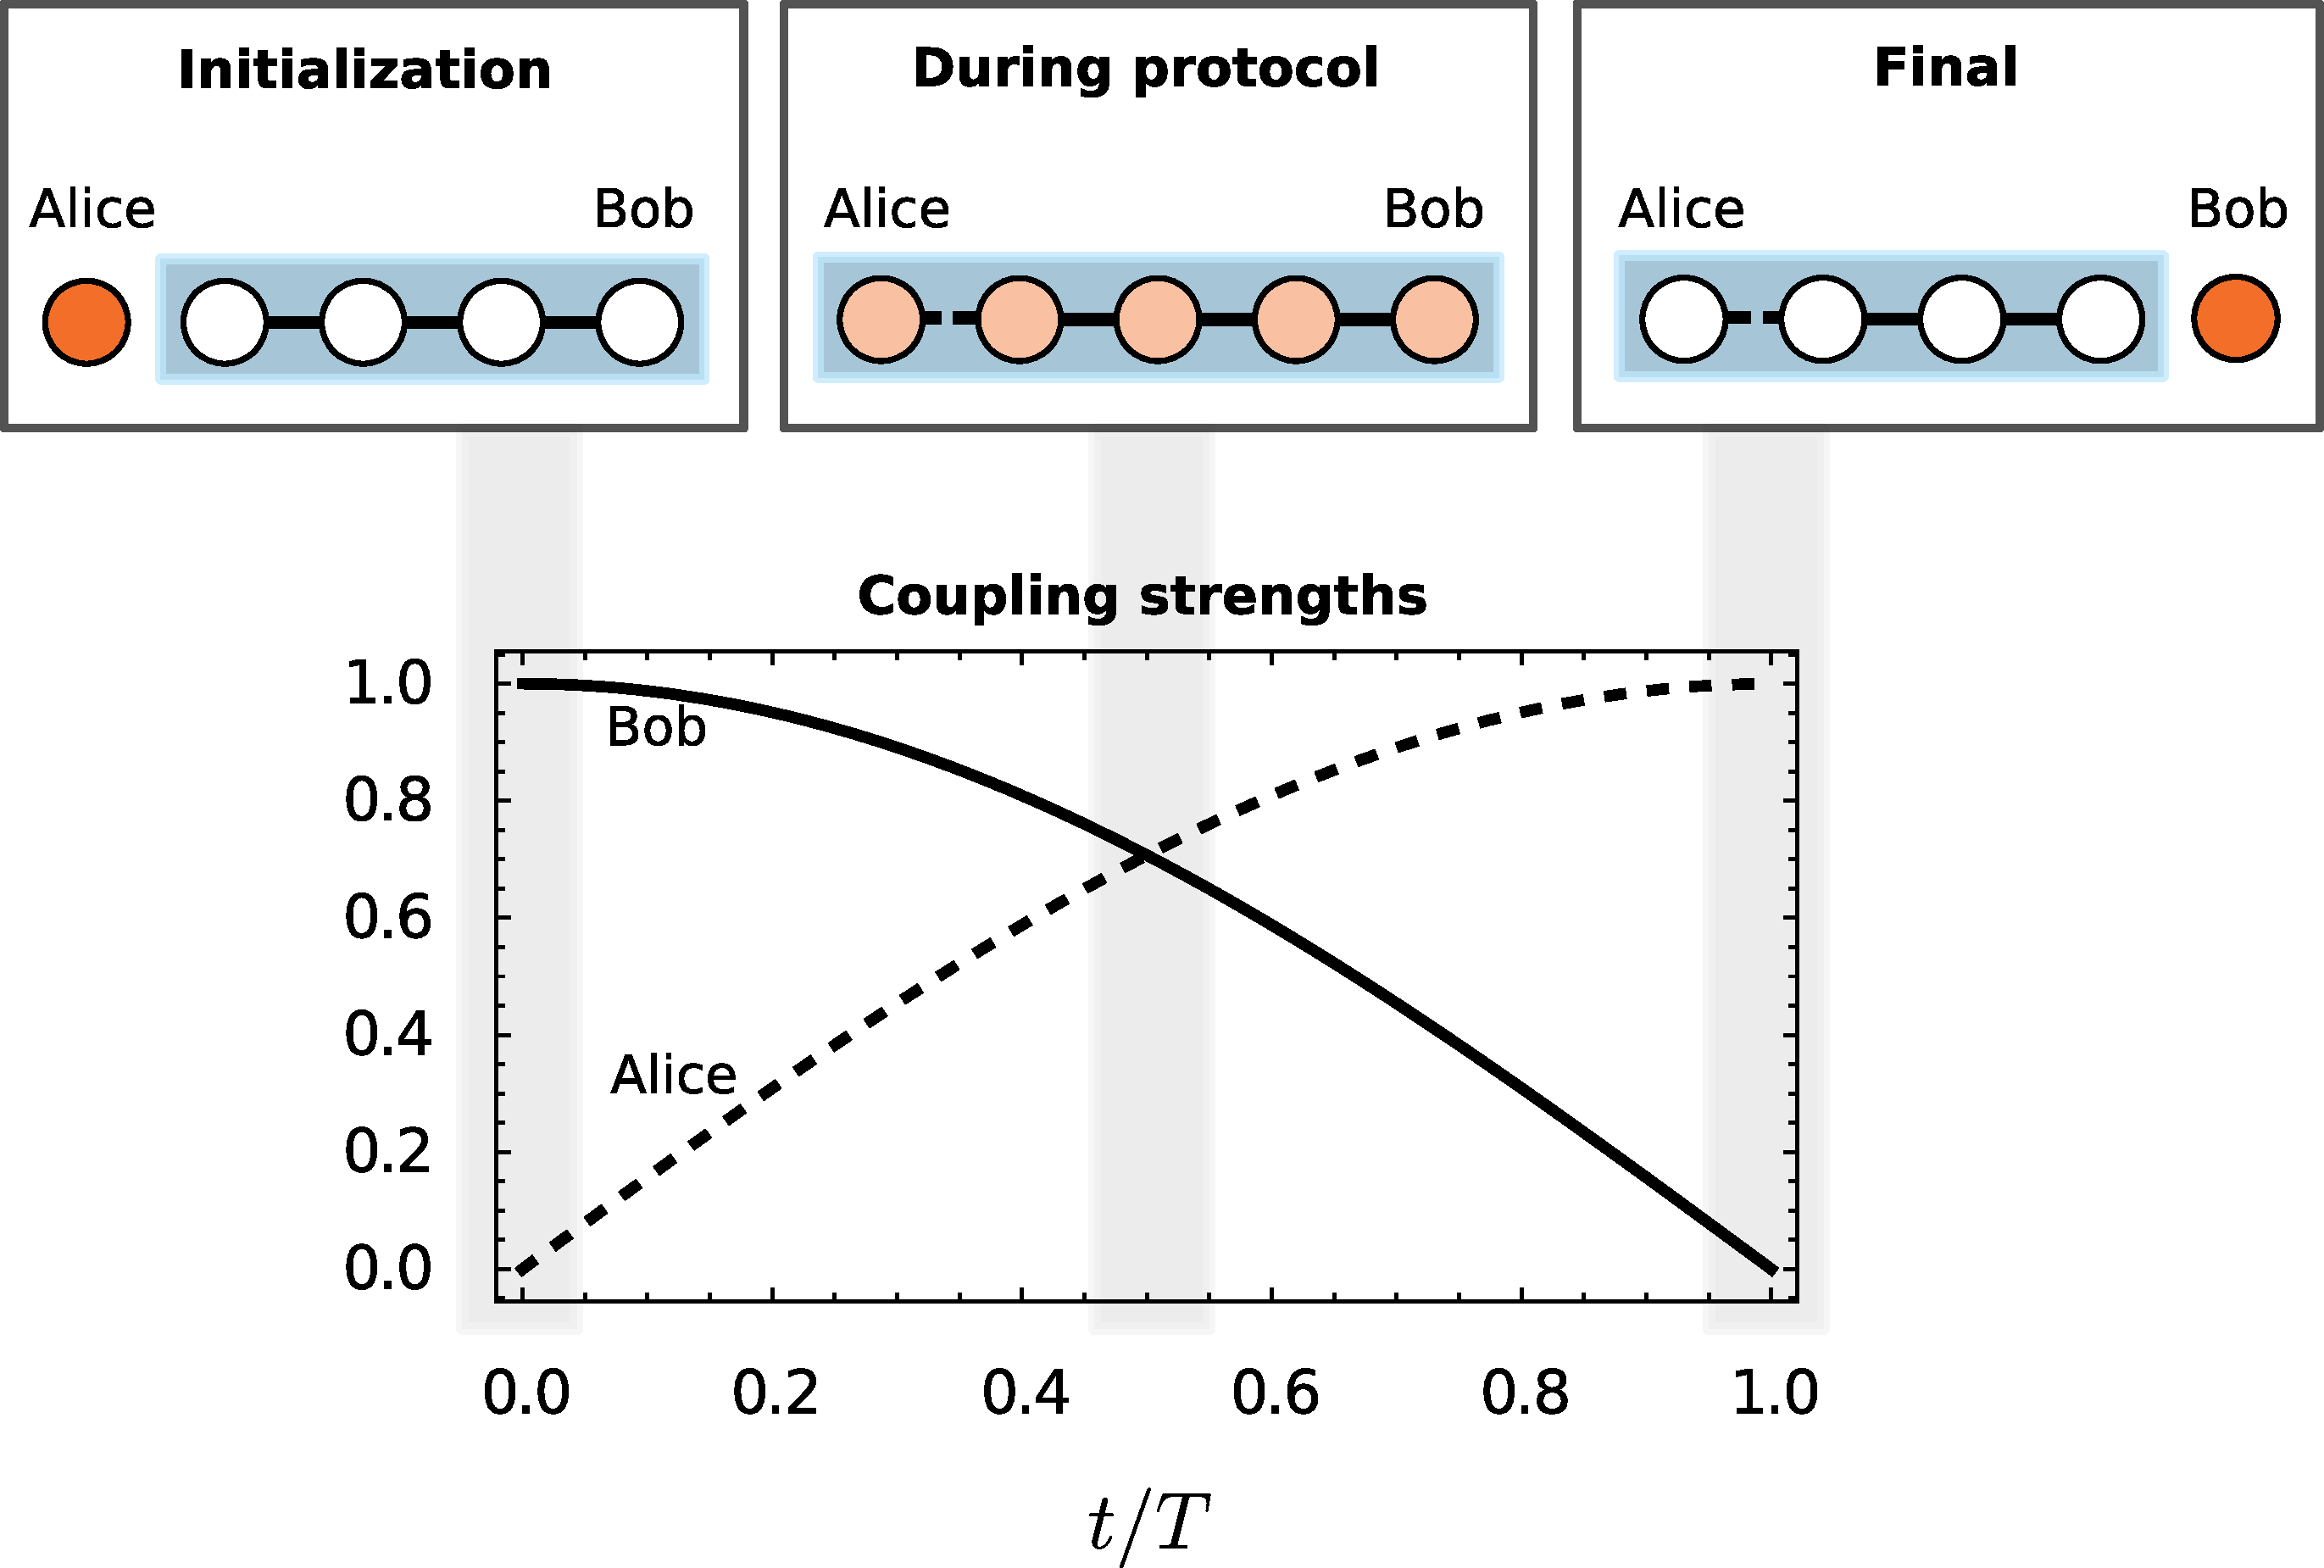
\includegraphics[width=.7\textwidth]{./img/adiabatic_protocol_sketch_v2.pdf} 
\end{center}
\caption{A sketch of a typical adiabatic transfer protocol, with the counter-intuitive pulse sequence. The top row indicates the initial, midway and final step of the protocol on a 5-site chain, with black lines representing the  coupling strengths $W_{j,j+1}$. The blue contour indicates which sites are coupled. The bottom graph shows a possible trajectory for Alice's couplings $W_{aj}$ and Bob's couplings $W_{bj}$.  }
\label{fig:adiabatic_protocol_sketch}
\end{figure}


Although these protocols are inherently slower than quenches, adiabatic protocols are often easier to implement experimentally because no precise timings are required, and because they are relatively resilient to decoherence and random or systematic errors in the control fields \cite{Childs2001, Farooq2015}. 

%


One of the most studied adiabatic transfer techniques is STImulated Raman Adiabatic Passage (STIRAP), which considers three internal states of an atom, of which the only possible couplings are $1 \leftrightarrow 2$ and $2 \leftrightarrow 3$ \cite{Gaubatz1990}. For our purposes, this is essentially a chain of length $3$, and indeed, the protocol was later extended allow transfer between the ends of a chain of any (odd) length $N$ \cite{Malinovsky1997}. The protocol follows precisely the counter-intuitive sequence described above, and we will study it in more depth in \cref{chap:ctap}. The atomic levels may not quite count towards \emph{spatial} transfer, but the model takes precisely the form of \cref{eqn:Hpst} where $W$ is the adjacency matrix of a chain, and the same mathematics have indeed been applied in spatially extended systems. These include an electron hopping over quantum dots \cite{Greentree2004} (where it is called Coherent Tunneling by Adiabatic Passage (CTAP)), cold atoms hopping through optical traps \cite{Eckert2004}, or a single (higher) spin excitation in the XXX \cite{Batey2015} and XX model \cite{Ohshima2007,Greentree2014} (where it is called Dark Passage).


Apart from STIRAP-based protocols, there are various variations of adiabatic transfer, most notably transfer in slightly different particle hopping chains \cite{Chen2012,Gratsea2018}.



\subsection{Half filling}
\label{sec:transport-half-filling}
Having considered ferromagnetic spin models, we treat the anti-ferromagnetic variants in a similar fashion. In this case, Alice may initialize the system's state as
\begin{align}
\ket{\Psi(0)} = \left( \alpha \ket{0} + \beta \ket{1} \right)_a  \otimes \ket{ \text{rest} },
\label{eqn:transferpsi0}
\end{align}
where $\ket{\text{rest}}$ is generally taken to be the ground state of the Hamiltonian restricted to the graph $G-a$. 
We typically assume conservation of number of excitations, and that the AFM ground state can be found in the sector with roughly $N/2$ excitations, hence the name \emph{half filling}. To be precise, if we assume $N$ odd, then $\ket{\text{rest}}$ is a state on $N-1$ qubits with $\frac{N-1}{2}$ spin excitations. Then, the evolution of $\ket{\psi(t)}$ takes place in two excitation sectors, namely those with $\lceil \frac{N}{2} \rceil$ and $\lfloor \frac{N}{2} \rfloor$ excitations. In the case of particle-hole symmetry, i.e. $[H,X^{\otimes N}]=0$, these sectors will evolve similarly. At any stopping time $T$, the mixed state $\rho_B$ that Bob receives is found by tracing over all sites $V$ except for Bob's:
\begin{align*}
\rho_B = \text{tr}_{V - B} \big( \ket{\Psi(T)} \bra{\Psi(T)} \big)
\end{align*}
Note that in this setting, compared to the single-excitation case, the dimensions of the relevant subspaces increases from $N$ to ${ N \choose \lceil N/2 \rceil }$, which is a dramatic increase in size. This makes the task of state transfer more difficult in this setting, and various techniques in many-body physics may be required.

\paragraph{Quench}
Quenches on half-filled systems are very common in condensed matter literature, but quenches in the context of state transfer less so. 
We already saw that certain open spin chains that allow PST or mirror inversion in the single-excitation sector, also allow transfer in higher excitation sectors. In particular, for XX chains such as the Krawtchouk chain, the mapping to non-interacting fermions makes it clear that results about single particle transfer still hold in the case of half-filling, up to signs. 

Campos Venuti et al. study quenched transfer in the XXX model with spin-$\frac{1}{2}$ and spin-$1$ particles  \cite{CamposVenuti2007}. As they indicate, the dispersion of this AFM model is actually linear at low energies, which is very distinct from the FM case, where the dispersion is quadratic. The findings are that quenched transfer can take place in a chain, with reasonable fidelities, as long as the \emph{outer} qubits are much more weakly coupled than the qubits in the bulk of the chain. We will refer to engineering such a relatively weak coupling at certain sites as \textbf{straddling}. 


\paragraph{Entanglement}
The case of half-filling is endowed with many results that are technically not about state transfer, but deal with emerging long-distance entanglement. Many of these results will turn out to be useful later in this thesis. 

The straddled XXX chain that allows quenched transfer happens to also feature strong entanglement between the more weakly coupled sites, when cooled to its ground state \cite{CamposVenuti2006, CamposVenuti2007}. In the limit of asymptotically strong straddling, the ground state takes the form of a maximally entangled state on the straddled sites, even if particles have higher spin.  In \cref{chap:heisenberg}, we will see that this generalizes to certain other bipartite graphs \cite{Groenland2019}.

Similar straddling effects are found in the AFM XX chains. In fact, one may perform a second iteration of attaching \emph{even more weakly coupled} qubits to the ends of the chain, which in turn form a strongly entangled pair. Performing multiple iterations, one may obtain a chain where the couplings decay exponentially towards the left and right, such as  \cite{Vitagliano2010,Ramirez2018}
\begin{align*}
H = \sigma_{\frac{1}{2}}^+ \sigma_{-\frac{1}{2}}^- +  \sum_{j=\frac{1}{2}}^{\frac{N-3}{2}} e^{-h j} \left[ \sigma_j^+ \sigma_{j+1}^- + \sigma_{-j}^+ \sigma_{-(j+1)}^- \right] + h.c.,
\end{align*}
where the site indices run from $-\frac{N-1}{2}$ to $\frac{N-1}{2}$. With increasing $h$, the ground state becomes asymptotically close to a so-called \textbf{rainbow state}, referring to the rainbow pattern that one obtains when drawing an arc between each qubit and its entangled partner. 
Finding a rainbow state as a ground state of a 1D chain is somewhat surprising: it has asymptotically $N/2$-qubit entanglement between its left and right halve, even though local 1D chains are expected to adhere to some area law \cite{Eisert2010}. The catch here is that the couplings are exponentially varying, which is an unrealistic assumption in the thermodynamic limit. 

The rainbow state has connections to other models in this thesis. In fact, a quench by the aforementioned Krawtchouk chain does not only perform a perfect mirror inversion after time $T$ (even when the initial state is the AFM ground state), but it also maps an initial N\'{e}el state $\ket{0101\ldots}$ to a rainbow state after a quench time $T/2$ \cite{Alkurtass2014}. 

Another interesting fact, which, to my best knowledge, has never been published, is that every \emph{mirror-symmetric} XX spin chain without local fields has a rainbow state as eigenstate in the middle of its spectrum. This can be proven by a symmetry argument, and is best explained by first mapping to the equivalent fermionic hopping model\footnote{Many thanks to Freek Witteveen for pointing this out to me.}. 
Assume that, within a certain symmetry sector $F$, all fermionic modes are filled, and all other modes are empty. For this special state, it does not matter in which fermionic basis (here $c$ or $d$) the occupation numbers are written: either way, the state contains all modes in $F$ anyway,
\begin{align*}
\ket{\Psi} = \prod_{c^\dagger_j \in F} c_j^\dagger \ket{0} \propto  \prod_{d^\dagger_j \in F} d_j^\dagger \ket{0} 
\end{align*}
In our case, we use the left-right mirror symmetry of the chain to guarantee that the system block-diagonalizes into an even and an odd part. We can choose $F$ to be the \emph{odd} block, such that $\{ ~ c^\dagger_j \ket{0} ~ | ~ c^\dagger_j \in F ~ \}$ are odd single-particle eigenstates, which have an eigenvalue $-1$ when acted on by the operator that sends $j \rightarrow N-j+1$\footnote{Note the subtle difference between the symmetry operation of relabeling the sites ($j \rightarrow N-j+1$) that is relevant to the \emph{left-right symmetric}  chain, as opposed to the sign related to the exchange of fermionic particles, which holds for \emph{any} fermionic system.}.
Then, $\ket{\Psi}$ is the unique eigenstate that contains all odd modes (and no even modes). Moreover, we can choose $d^\dagger_j = \frac{1}{\sqrt{2}} \left( f^\dagger_j - f^\dagger_{N-j+1} \right)$ to be another basis of anti-symmetric states, where $f^\dagger_j$ are again the \emph{local} operators, creating a fermion at site $j$. Adding each of these states to the system gives rise to a state identical to $\ket{\Psi}$, up to a global phase. Now, mapping back to a spin model through the JW transform, this state becomes
\begin{align*}
\ket{\Psi'} \propto \prod_{j=1}^{N/2} \left( \sigma_j^+ + (-1)^j \sigma_{N-j+1}^+ \right) \ket{0}
\end{align*}
This is precisely a rainbow state, and we showed that it is an eigenstate of the symmetric XX chain. A similar result holds for the \emph{even} sector. Lastly, we note that this state is always in the \emph{middle} of the spectrum of the system: in a symmetric chain without local fields, the single-particle spectrum is symmetric around zero, and increasing energies alternatingly correspond to even and odd states. Therefore, for odd $N$, the two Rainbow eigenstates both have precisely zero energy. For even $N$, energies of the `even' and the `odd' rainbow states are nonzero, but relatively small, and differ from each other by a sign. 



\paragraph{Adiabatic}
Adiabatic transfer in anti-ferromagnetic models received quite some scientific attention, partially because coupled quantum dots, with a single electron per dot, approximately form an AFM XXX model. Various models have been studied, such as the Heisenberg model \cite{Farooq2015,Agundez2017,Groenland2019}, the $J_1 - J_2$ model \cite{Chancellor2012}, spin-1 particles with generalized bilinear–biquadratic Heisenberg interaction \cite{Eckert2007}, and the XXZ model \cite{Oh2013}. 

As in the ferromagnetic case, a typical adiabatic protocol is supposed to start and end such that the sending/receiving site is an eigenstate of the Hamiltonian. Indeed, each of the references in the previous paragraph uses the counter-intuitive pulse sequence, or a slight variations thereof. 

As with quenches, the huge dimensionality of the half-filled case makes analysis of the models rather hard. In \cref{chap:heisenberg}, we will discuss transfer in the XXX model, relying heavily on the theory presented in \cref{sec:XXXmodel}.
 
%


\subsection{Transfer on graphs that are not chains}
\label{sec:transfergeneralgraphs}
Most results quoted in this section deal with the transfer of states over linear chains. From a practical point of view, this makes much sense: a chain is the graph with the highest ratio between diameter and number of sites, connecting two endpoints with as few sites as possible. Still, various applications may require state transfer over more general graphs, such as networks where multiple parties are strongly coupled at all times. As an example, Vandersypen et al. \cite{Vandersypen2017} consider future challenges in scaling up quantum computers based on electron spin qubits in quantum dots. They find that individual arrays of qubits need to be placed in vicinity of classical hardware that is responsible for control tasks, such as gate pulses and measurements. They sketch a computer chip design where a large number of `qubit islands' are connected with long range couplers, such that other electronics can be placed in between the islands. Such designs could greatly benefit from more flexible coupling methods, where all islands could be connected to the same network, rather than placing an individual coupler between every nearby island. Similar reasoning may hold for other platforms as well. Still, results on non-chain graphs seems surprisingly scarce, and we will discuss the known results throughout this subsection. 

By far the most results on non-chain graphs can be found in the context of perfect state transfer (using quenches on single-excitation systems). The field of algebraic graph theory chases a main question of characterzing graphs that allow PST, leading to a plethora of results \cite{Bachman2011}. Various classes of graphs are known to exhibit state transfer \cite{Bernasconi2008,Basic2009,Cheung2011}, and various graph properties can be linked to the absence or presence of state transfer \cite{Godsil2012,Bachman2011}. 


Some results are known in the adiabatic variant of the single-excitation transfer, particularly in the context of CTAP. Longhi generalizes the chain-based transfer of quantum particles to transfer between the opposite corners of a square grid in any dimension \cite{Longhi2014}. The result uses a smart decomposition of the grid into individual 1D chains, each of which requires a standard STIRAP/CTAP protocol for the transfer. In the same work, Longhi presents a transfer scheme on a triangular lattice, cut in the shape of a triangle, where CTAP is possible using specifically engineered couplings. The scheme works thanks to an earlier results by Bradly et al. \cite{Bradly2012}, who consider the transfer of $N$ bosonic particles hopping between three coupled sites. 
The states of this space can be represented using two parameters $n_1, n_2$ as $\ket{ n_1, n_2, N-n_1 - n_2 }$, and Bradly et al. present a scheme that adiabatically maps a state $\ket{N, 0, 0}$ to the state $\ket{0,N,0}$. The same states, however, can be interpreted as sites on a two-dimensional lattice $\ket{n_1, n_2}$, whose couplings are given by the bosonic hopping amplitudes. These couplings do not only give the triangular connectivity, but also form Krawtchouk chains along the main directions of the grid, the very same that we discussed earlier in this section. 

Another interesting CTAP result that involves more than just a linear chain is by Greentree et al. \cite{Greentree2006}, who consider multiple receivers dangling along the odd sites of a linear chain, along with a sender dangling along site $1$. Within this configuration, the amplitude of the sender can be transported to any one of the receivers. Other works, such as Refs. \cite{Chen2013,Batey2015}, describe a variation where the chain splits into multiple paths or branched endpoints. The extension to these graphs is not surprising because these systems can be mapped back to a linear chain by symmetries. However, interesting physics can be observed when the transferred state is sent to multiple symmetric receivers, such that the final state forms a superposition between the various endpoints. 

Apart from these results, I am not aware of any documentation of state transfer on general graphs, outside of the PST setting. Two of the main results of the thesis, presented in \cref{part:adiabatic}, deal with adiabatic transfer on more general graphs. One of our results deals with CTAP and STIRAP, in which we consider a class of graphs much larger than those presented in the previous paragraphs (\cref{chap:ctap}). The other results deals with the AFM XXX model, which is to my best knowledge the only result of state transfer in truly non-chain graphs in the setting of half filling (\cref{chap:heisenberg}). 

Looking at \cref{tab:transfer}, it seems that some models have not had a general graph treatment yet, which may be interesting directions for future research. In particular, this includes quenches on half-filled systems, but also adiabatic transfer in the \emph{single-excitation} Ising and XXX model. I don't know how to tackle the first or second case, but there is much to say about the third.

\paragraph{Musings on adiabatic transport in the FM XXX model} The Hamiltonian of an XXX model, restricted to a single spin up, takes the form of the Laplacian matrix of the model's graph, $H = L_G = D_G - A_G$. It is not hard to check that all eigenvalues of $L_G$ are either $0$ or positive, and the multiplicity of the zero eigenvalue is equal to the number of connected components. The good news is that, in this settings, we always find a unique ground state with energy precisely $0$, regardless of the graph, as long as it is \emph{connected}. The bad news is that, once we disconnect Alice or Bob from the graph, the ground state becomes degenerate, possibly jeopardizing the adiabatic process. If only we had a way to overcome this degeneracy, we would find that adiabatic transfer works in \emph{any} graph of this model! One potential solution is the following: if we allow ourselves the use of inhomogeneous local fields, of the form $H' = \sum_{j} B_j Z_j$, the we can make sure that the disconnecting party always has a \emph{lower} energy than the ground state of the main connected component. Simply setting $B_j < 0$ for the connecting party $j$ and $B_{k} > 0$ for all other parties $j\neq k$ would be sufficient. Realizing such inhomogeneous magnetic fields at the scale of inter-spin distances is experimentally challenging, and studying the viability of this protocol would be an interesting direction of future research. 



















%

%
%
%
%
%
%
%
%
%
%
%
%
%



